\chapter{Laboratorio 5: \\Leakage: using spice for characterizing cells and pen\&paper for memory organization}
In questo laboratorio viene richiesto di analizzare i contributi di potenza, prestando particolare attenzione particolarmente alla potenza di leakage.

\section{Characterizing a library gate}
In questa prima parte dell'esercitazione viene richiesto di analizzare le performance di una \textit{NAND} a due ingressi, ottimizzata per essere \textit{High-Speed} per avere esattamente un punto di riferimento quando si analizzerà il caso con basso leakage. La porta NAND in questione si compone di due pMOS in parallelo, collegati alla Vdd e due nMOS in serie collegati al GND, come si può osservare in Figura \ref{nand_circuit}. \\
\begin{figure}[!htb]
	\centering
	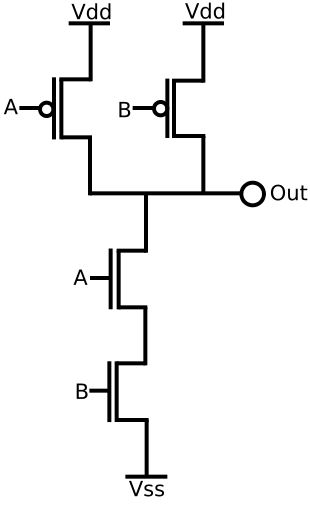
\includegraphics[scale=0.3]{immagini/nand_circuit}
	\caption{\textit{Schema interno porta NAND}}
	\label{nand_circuit}
\end{figure}
La definizione del pMOS e dell'nMOS avviene tramite una piccola libreria \textit{'CMOS2013'}, all'interno della quale sono definiti i modelli che verranno analizzati (nel nostro caso si tratta del \textbf{EPHSGP\_BS2JU} per il pMOS e \textbf{ENHSGP\_BS2JU} per l'nMOS). All'interno di questa libreria ogni transistore viene identificato tramite alcuni parametri, quali la lunghezza e la larghezza del MOS e perimetri e aree di draine source.
L'analisi avviene tramite uno script \textit{'nandHS.sp'} che contiene una netlist dove vengono fissati i valori dei parametri di larghezza e lunghezza dei transitori.\\
Inoltre lo script contiene anche il comando .measure tramite il quale vengono stimati i tempi di salita, di discesa e di propagazione della porta in questione. Viene richiesto di completare questi comandi andando a scrivere un comando per la misura tel tempo di propagazione basso-alto. Il comando aggiunto in questione è il seguente:
\begin{center}
\textit{.measure tran nanddelayHL TRIG V(inB) VAL='alim*0.5' RISE=1 
+ TARG V(out) VAL='alim*0.5' FALL=1}
\end{center}
Settando l'ambiente di simulazione \textbf{ELDO}, si può procedere con la simulazione della NAND in questione andando a riportare i parametri richiesti dalla traccia. Tra tutti i parametri viene richiesto di annotare la potenza totale dissipata, che risulta essere pari a 6.7908 nW. I risultati temporali invece sono riportati in Tabella \ref{Tab5_1}.\\
\begin{table}[!h]\footnotesize
	\centering
	\begin{tabular}{|c|c|}
		\hline
		\textbf{Tempo} & \textbf{Misura}\\
		\hline
		$t_{rise}$ & 89.303 ps\\
		$t_{fall}$ & 74.319 ps\\
		$t_{pdHL}$ & 48.993 ps\\
		$t_{pdLH}$ & 56.490 ps\\
		\hline
	\end{tabular}
	\caption{\textit{Risultati tempi NAND simulazione ELDO}}
	\label{Tab5_1}
\end{table}
\\
Si possono confrontare questi valori andando ad avviare una simulazione grafica tramite \textbf{ezwave}. Le onde risultati sono riportate in Figura \ref{onde_5_1}, dove sono riportati i valori delle due tensioni di ingresso che, come visto dalla netlist, risultano essere:
\begin{itemize}
	\item INA: costante al valore 1.2 V, assimilato come '1' logico
	\item INB: 0 V fino ad 1 ns, 1.2 V fino a 2 ns, 0 V fino al termine della simulazione
\end{itemize}
\begin{figure}[!htb]
	\centering
	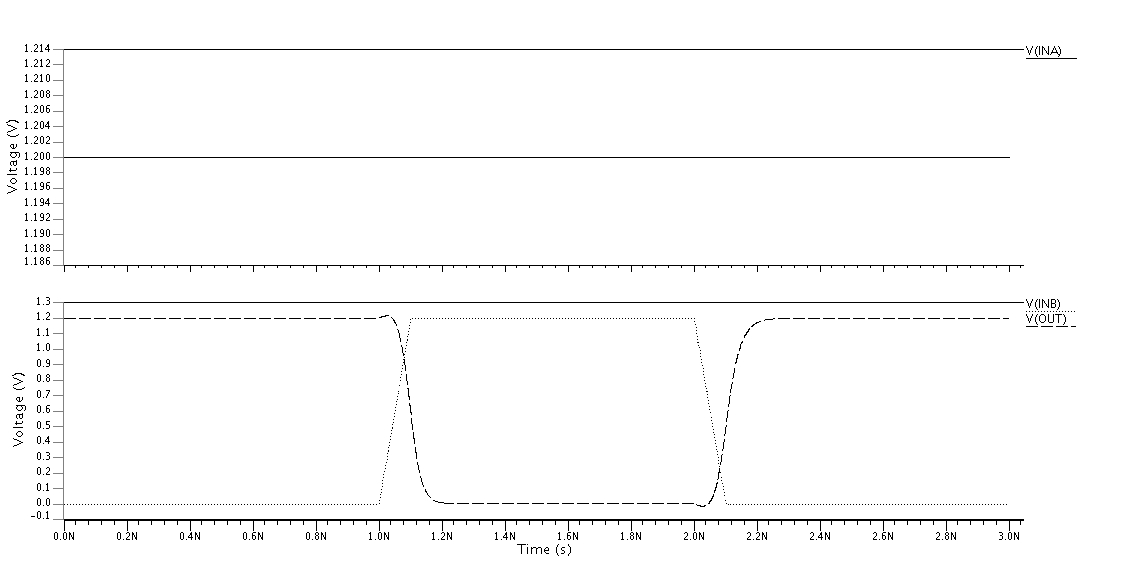
\includegraphics[scale=0.35]{immagini/onde_5_1}
	\caption{\textit{Onde delle tensioni di ingresso}}
	\label{onde_5_1}
\end{figure}
Tramite gli appositi cursori del programma sono stati ricavati i tempi calcolati in precedenza con ELDO. Tutti i tempo sono riportati i Tabella \ref{Tab5_2}. 
\begin{table}[!h]\footnotesize
	\centering
	\begin{tabular}{|c|c|}
		\hline
		\textbf{Tempo} & \textbf{Misura}\\
		\hline
		$t_{rise}$ & 84.64 ps\\
		$t_{fall}$ & 74.01 ps\\
		$t_{pdHL}$ & 47.24 ps\\
		$t_{pdLH}$ & 56.71 ps\\
		\hline
	\end{tabular}
	\caption{\textit{Risultati tempi NAND simulazione ezwave}}
	\label{Tab5_2}
\end{table}
\\
Si può ben notare come i risultati siano assolutamente confrontabili.\\
In seguito viene chiesto di fare un'analisi in continua, andando a decommentare alcune linee dello script, per andare a valutare le tensioni di soglia dei diversi MOS. I risultati sono riportati in Tabella \ref{Tab5_3}. 
\begin{table}[!h]\footnotesize
	\centering
	\begin{tabular}{|c|c|}
		\hline
		\textbf{Transistore} & \textbf{Tensione di Soglia $V_{TH}$}\\
		\hline
		VT(XNAND.XMN0.M1) & 0.31371 V\\
		VT(XNAND.XMN1.M1) & 0.27241 V\\
		VT(XNAND.XMP0.M1) & -0.24712 V\\
		VT(XNAND.XMP1.M1) & -0.24712 V\\
		\hline
	\end{tabular}
	\caption{\textit{Tensioni di soglia}}
	\label{Tab5_3}
\end{table}.
\\
Ovviamente, come ci si aspettava, le tensioni di soglia dei pMOS sono negative, mentre quelle degli nMOS sono positive. Le due tensioni di soglia dei pMOS risultano identiche; non vale lo stesso nel caso degli nMOS, in quanto si ha che la tensione di soglia del MOS0 è superiore alla tensione di soglia del MOS1. Questo genera di conseguenza una corrente di leakage più alta nel caso del MOS1 rispetto al MOS0.

\section{Characterizing a gate for output load}
L'obiettivo di questa seconda sezione dell'esercitazione è di analizzare il funzionamento della porta NAND andando a variare il carico in uscita. Si analizzano i casi con carico pari a:
\begin{itemize}
	\item 0.005 fF
	\item 0.05 fF
	\item 0.5 fF
	\item 5 fF
	\item 50 fF	
\end{itemize}
A tale scopo si analizzata, sempre tramite l'ambiente di simulazione \textit{ELDO}, il file \textit{nandHScharLoad.sp}. Rispetto al file precedente viene inserita una misura per valutare i picchi di corrente che scorrono nel GND e nella capacità di carico. I risultati della simulazione sono contenuti nella Tabella \ref{Tab5_4} per i tempi e nella Tabella \ref{Tab5_5} per i risultati legati alla corrente.
\begin{table}[!h]\footnotesize
	\centering
	\begin{tabular}{|c|c|c|c|c|c|}
		\hline
		\textbf{$C_{Load}$} & \textbf{0.005 fF} & \textbf{0.05 fF} & \textbf{0.5 fF} & \textbf{5 fF} & \textbf{50 fF}\\
		\hline
		$t_{rise}$ &67.226 ps &67.604 ps &71.228 ps &102.81 ps &363.91 ps \\
		
		$t_{fall}$ &68.551 ps &68.830 ps &72.112 ps &98.194 ps &296.52 ps \\
		
		$t_{pdHL}$&20.524 ps &20.851 ps &23.980 ps &48.550 ps &180.16 ps \\
		
		$t_{pdLH}$ &37.948 ps&38.286 ps &41.521 ps &66.657 ps &209.00 ps \\
		
		\hline
	\end{tabular}
	\caption{\textit{Risultati tempi NANd simulazione ELDO}}
	\label{Tab5_4}
\end{table}
\begin{table}[!h]\footnotesize
	\centering
	\begin{tabular}{|c|c|c|c|c|c|}
		\hline
		\textbf{$C_{Load}$} & \textbf{0.005 fF} & \textbf{0.05 fF} & \textbf{0.5 fF} & \textbf{5 fF} & \textbf{50 fF}\\
		\hline
		$I_{GND, f}^{max}$ &76.530 $\mu$A &77.056 $\mu$A &81.964 $\mu$A &116.64 $\mu$A &240.77 $\mu$A \\
		
		$I_{Vdd, r}^{max}$ &-70.006$\mu$A &-70.423 $\mu$A &-74.383 $\mu$A &-102.77 $\mu$A &-209.19 $\mu$A \\
		
		$I_{GND, r}^{max}$&45.879 $\mu$A &45.692 $\mu$A &44.055 $\mu$A &34.693 $\mu$A &12.571 $\mu$A\\
		
		$I_{Vdd, f}^{max}$& -47.912 $\mu$A&-47.680 $\mu$A &-45.637 $\mu$A &-34.365 $\mu$A &-11.039 $\mu$A \\
		
		$I_{Load, f}^{max}$ &8.2877 nA &8.2877 nA &8.2877 nA &8.2893 nA &372.90 nA \\
		
		$I_{Load, r}^{max}$ &-5.6590 nA &-5.690 nA &-5.6590 nA &-5.6734 nA &-12.547 nA \\
		\hline
	\end{tabular}
	\caption{\textit{Risultati simulazione ELDO delle correnti}}
	\label{Tab5_5}
\end{table}
\\
Analogamente al punto precedente, si è sfruttato \textit{ezwave} per andare a plottare gli andamenti delle tensioni e delle correnti al variare del carico. I risultati sono riportati in Figura \ref{onde_5_2current} per il caso delle correnti e in Figura \ref{onde_5_2voltage} per il caso delle tensioni.\\
\begin{figure}[!htb]
	\centering
	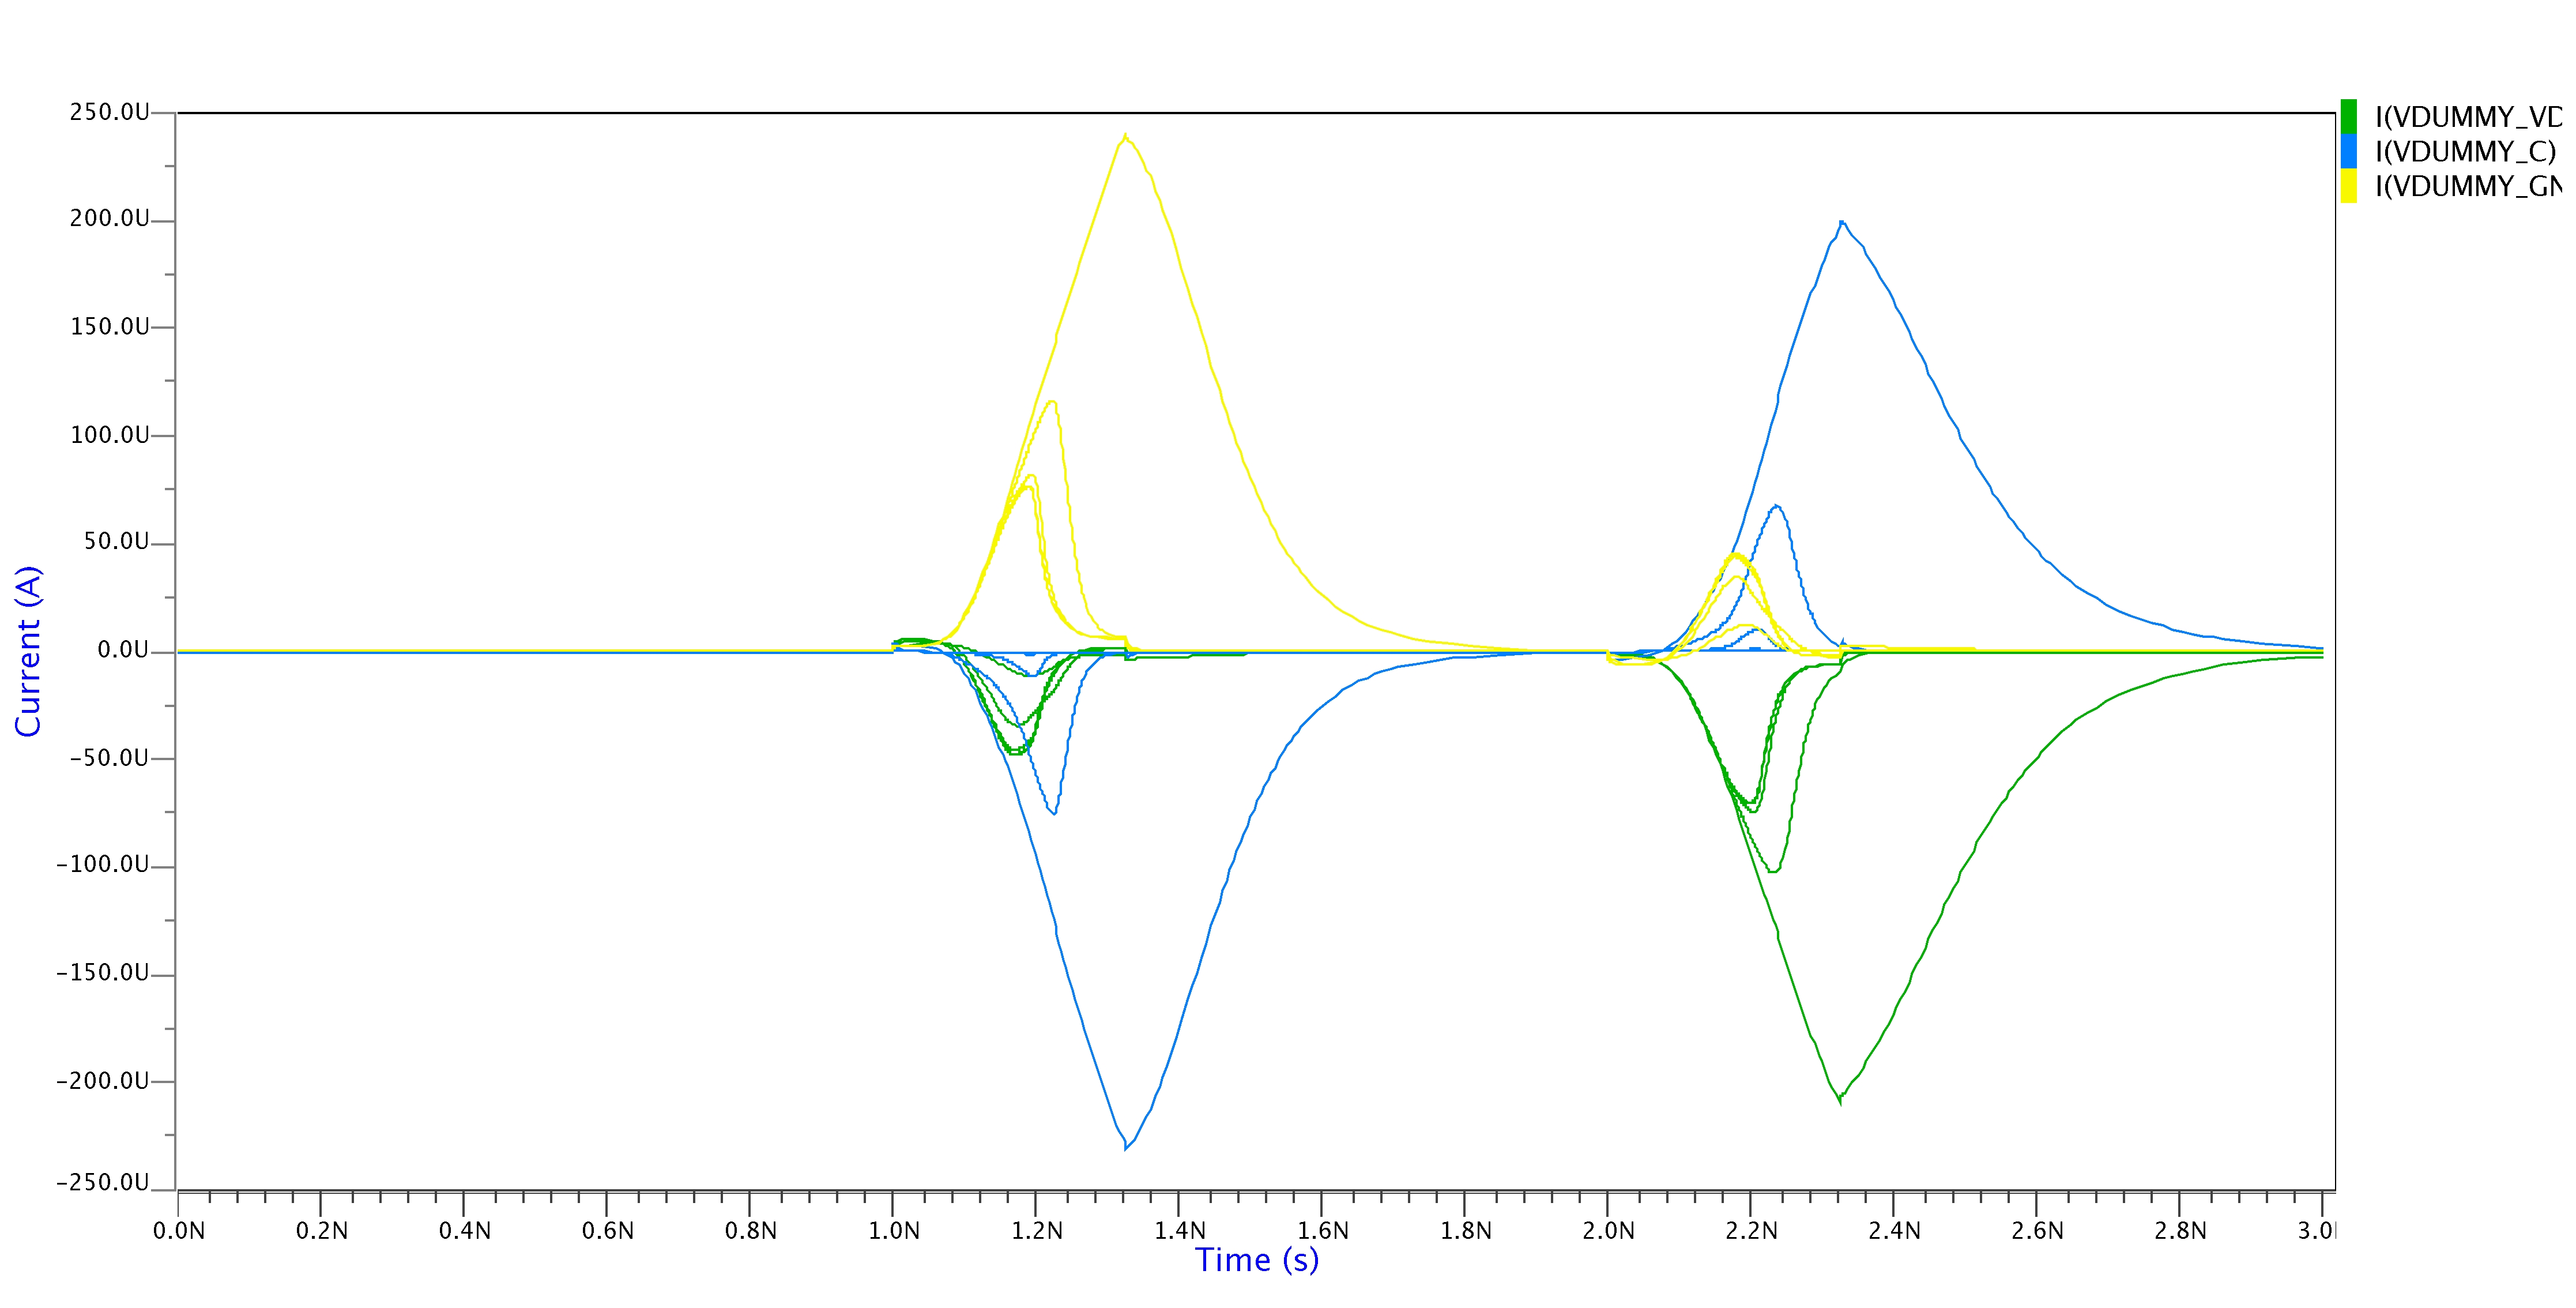
\includegraphics[scale=0.09]{immagini/onde_5_2current}
	\caption{\textit{confronto delle correnti}}
	\label{onde_5_2current}
\end{figure}
\begin{figure}[!htb]
	\centering
	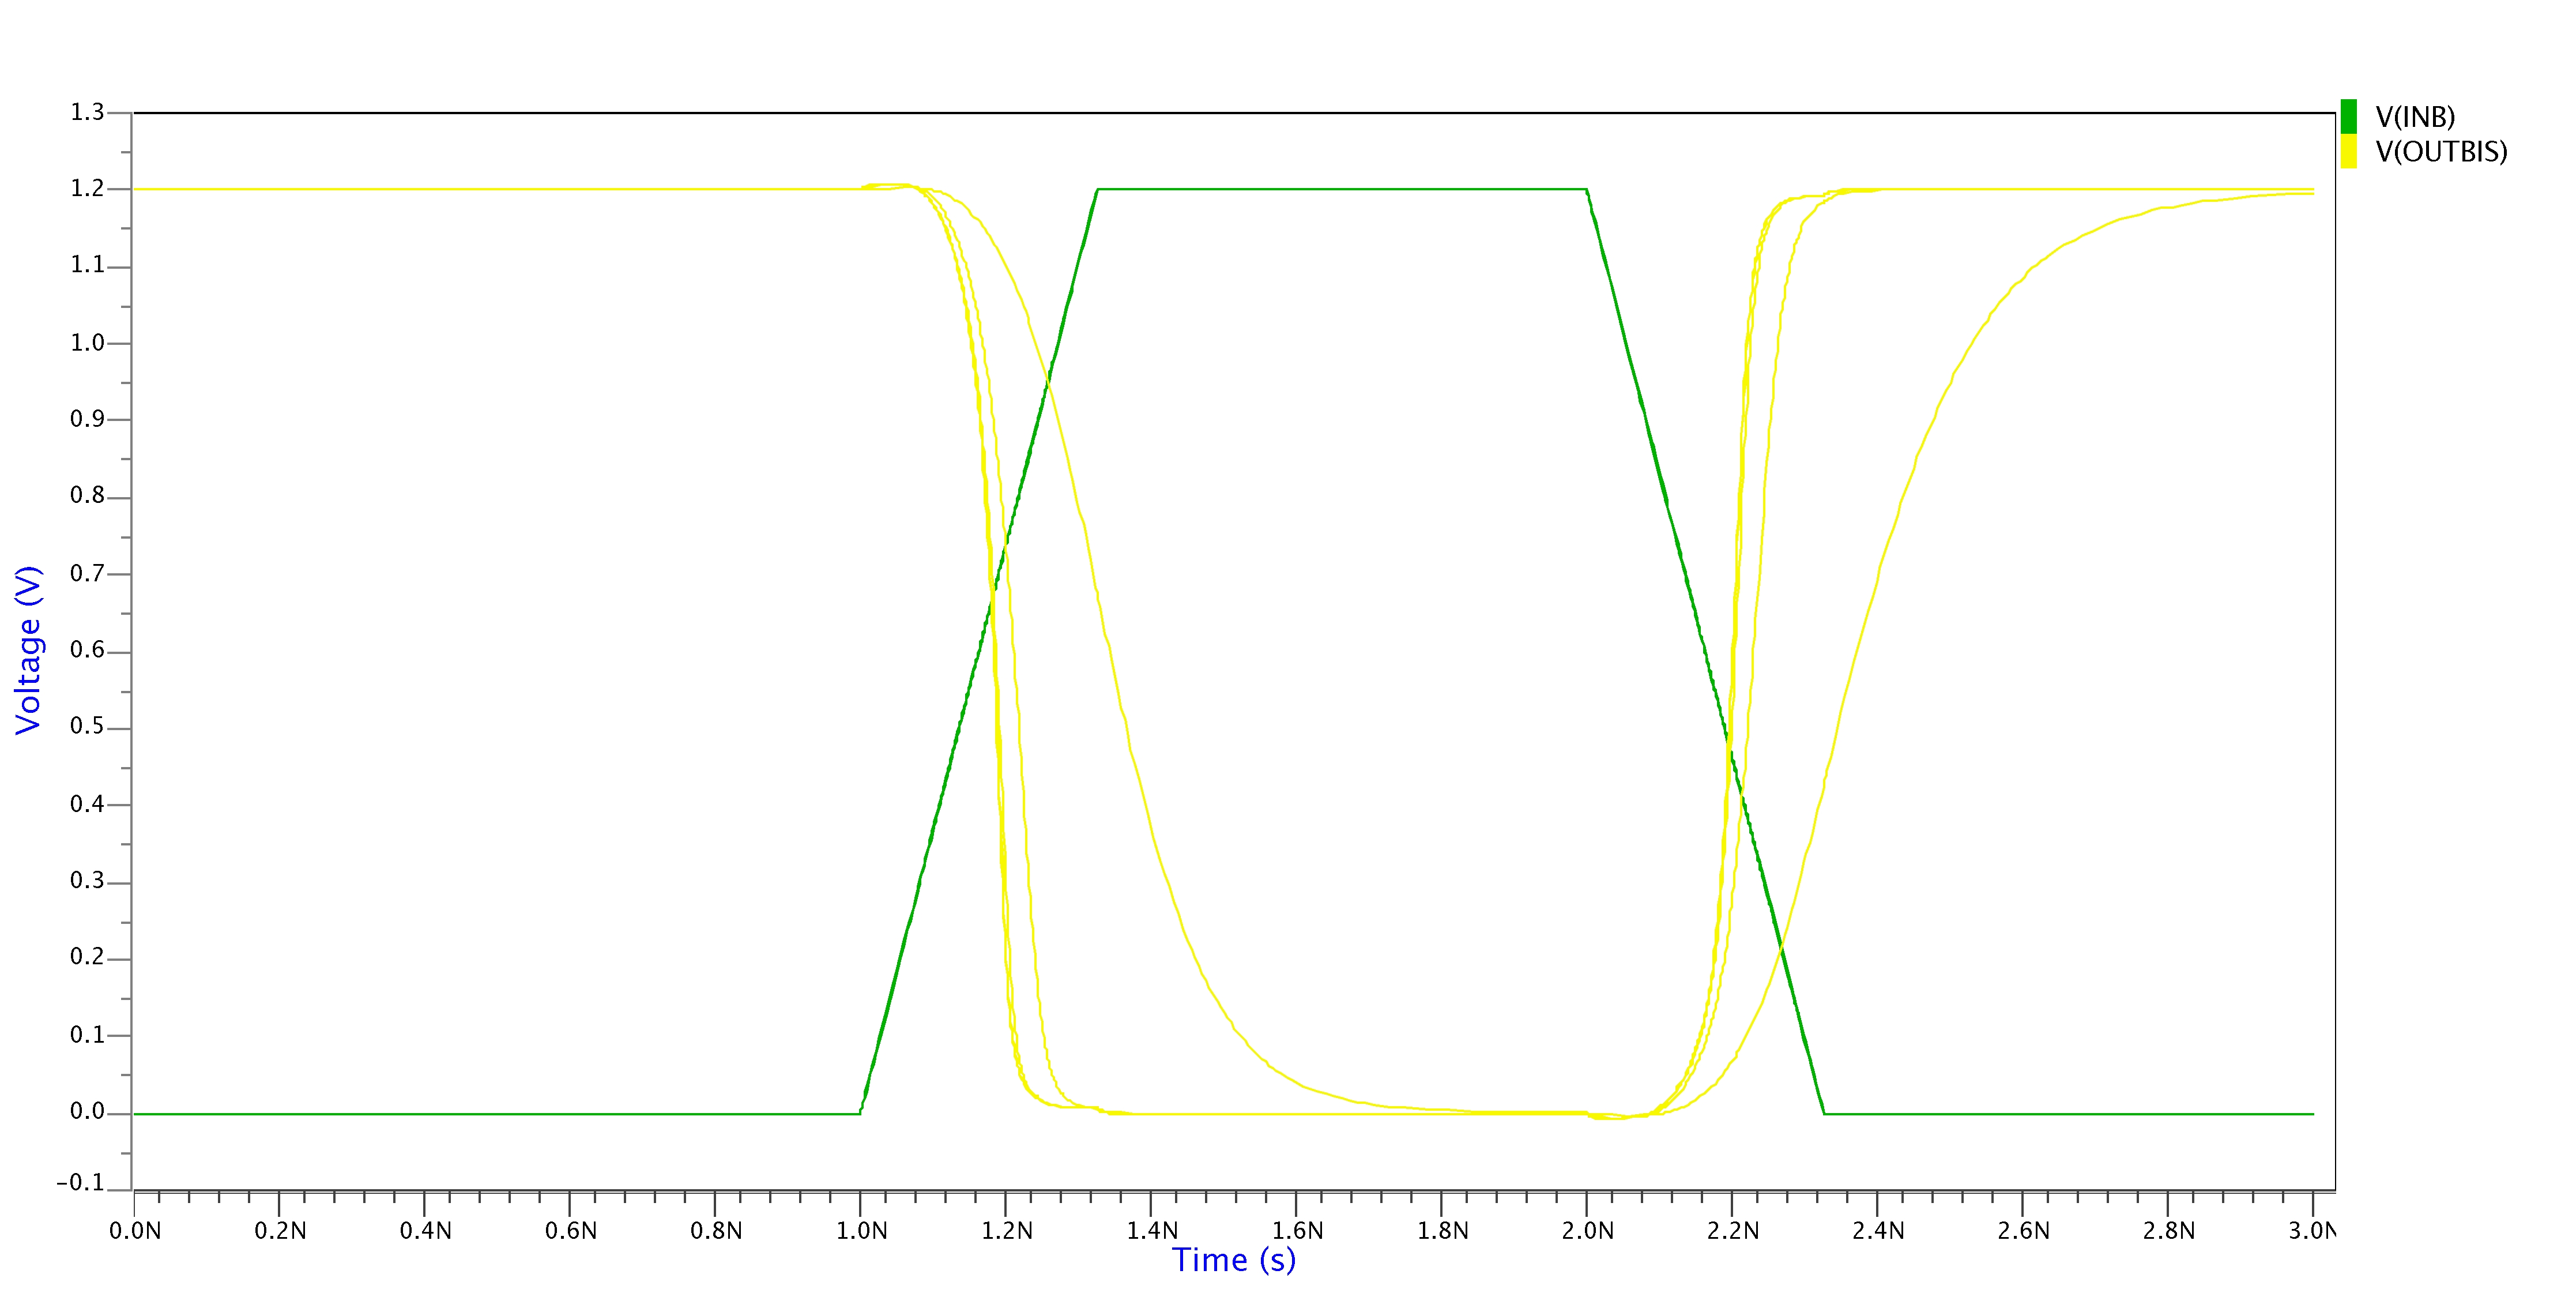
\includegraphics[scale=0.09]{immagini/onde_5_2voltage}
	\caption{\textit{Confronto delle tensioni}}
	\label{onde_5_2voltage}
\end{figure}
Si nota che all’aumentare del carico aumentano anche le transizioni in salita e discesa del segnale di uscita. Inoltre, si nota che avendo le variazioni del segnale di uscita più lente di quelle del segnale di ingresso, l’intervallo di tempo in cui le reti di pull-up e pull-down sono entrambe attive è minore: di conseguenza si avranno minori correnti di cortocircuito che causerebbero un significativo consumo di potenza. Dalla teoria si sa infatti che per avere consumi causati dalle correnti di cortocircuito bassi, gli slope del segnale di ingresso e di uscita devono essere quanto più simili possibili.
In modo analogo al caso precedente, si sono andate a calcolare le varie Tensioni di Soglia dei MOS. I risultati sono riportati nella Tabella \ref{Tab5_6}. \\
\begin{table}[!h]\footnotesize
	\centering
	\begin{tabular}{|c|c|c|c|c|c|}
		\hline
		\textbf{TRANSISTOR/$C_{Load}$} & \textbf{0.005 fF} & \textbf{0.05 fF} & \textbf{0.5 fF} & \textbf{5 fF} & \textbf{50 fF}\\
		\hline
		\textbf{XMN0.M1} &0.31371&0.31371&0.31371&0.31371&0.31371\\
		
		\textbf{XMN1.M1} &0.27241&0.27241&0.27241&0.27241&0.27241 \\
		
		\textbf{XMP0.M1}&-0.24712&-0.24712&-0.24712&-0.24712&-0.24712 \\
		
		\textbf{XMP1.M1}&-0.24712&-0.24712&-0.24712&-0.24712&-0.24712\\
			
			\hline
		\end{tabular}
		\caption{\textit{Tensioni di soglia}}
		\label{Tab5_6}
	\end{table}
\\
Esattamente come ci si aspettava, i valori delle tensioni di soglia sono identici rispetto al caso ottenuto nel paragrafo 5.1. Questo è dovuto al fatto che la $V_{TH}$ dipende esclusivamente dai parametri tecnologici con la quale viene realizzato il transistore e non ha alcuna dipendenza dal carico in uscita. 

\section{Comparing different gate sizing}
Le porte NAND analizzate fino ad ora erano ottimizzate per supportare carichi capicitivi che non superassero i 0.16 fF. Per avere dei gate ottimizzati per pilotare carichi superiori, bisgona utilizzare porte logiche differenti, comunque presenti nella libreria. \\
Viene chiesto di analizzare ora due porte NAND, di dimensioni differenti: una prima porta X1 ed una seconda porta, più grande della prima, denominata X8. Queste porte sono ottimizzate per pilotare carichi capacitivi fino ad un massimo di 1.28 fF. \\
Le due netlist contenenti le due diverse porte NAND sono: \textit{nandHScharMax\_Load.sp} e \textit{nandHSX8charMax\_Load.sp}. \\
Tutte le simulazioni vengono ora fatte utilizzando due carichi capacitivi diversi: 0.06 fF e 60.0 fF. I risultati nel caso della NAND X1 sono riportati nelle Tabelle \ref{Tab5_7} per i tempi e \ref{Tab5_8} per le correnti; mentre i risultati nel caso della NAND X8 sono riportati nelle Tabelle \ref{Tab5_9} per i tempi e \ref{Tab5_10} per le correnti.
\begin{table}[!h]\footnotesize
	\centering
	\begin{tabular}{|c|c|c|}
		\hline
		\textbf{NAND X1} & &\\
		\textbf{$C_{Load}$} & \textbf{0.06 fF} & \textbf{60 fF}\\
		\hline
		$t_{rise}$ &67.692 ps &425.04 ps  \\
		
		$t_{fall}$ &68.978 ps &341.77 ps  \\
		
		$t_{pdHL}$&20.923 ps &203.71 ps  \\
		
		$t_{pdLH}$ &38.361 ps&236.61 ps  \\
		
		\hline
	\end{tabular}
	\caption{\textit{Risultati tempi simulazione ELDO, NAND X1}}
	\label{Tab5_7}
\end{table}
\begin{table}[!h]\footnotesize
	\centering
	\begin{tabular}{|c|c|c|}
		\hline
\textbf{NAND X1} & &\\
\textbf{$C_{Load}$} & \textbf{0.06 fF} & \textbf{60 fF}\\
\hline
		$I_{GND, f}^{max}$ &77.172 $\mu$A &245.47 $\mu$A\\
		
		$I_{Vdd, r}^{max}$ &-70.514$\mu$A &-213.72 $\mu$A \\
		
		$I_{GND, r}^{max}$&45.653 $\mu$A &10.965 $\mu$A\\
		
		$I_{Vdd, f}^{max}$& -47.631 $\mu$A&-9.4773 $\mu$A \\
		
		$I_{Load, f}^{max}$ &8.2877 nA &1201.6 nA  \\
		
		$I_{Load, r}^{max}$ &-5.6590 nA &-19.994 nA  \\
		\hline
	\end{tabular}
	\caption{\textit{Risultati simulazione ELDO delle correnti, NAND X1}}
	\label{Tab5_8}
\end{table}
\begin{table}[!h]\footnotesize
	\centering
	\begin{tabular}{|c|c|c|}
		\hline
		\textbf{NAND X8} & &\\
		\textbf{$C_{Load}$} & \textbf{0.06 fF} & \textbf{60 fF}\\
		\hline
		$t_{rise}$ &67.692 ps &425.04 ps  \\
		
		$t_{fall}$ &68.978 ps &341.77 ps  \\
		
		$t_{pdHL}$&20.923 ps &203.71 ps  \\
		
		$t_{pdLH}$ &38.361 ps&236.61 ps  \\
		
		\hline
	\end{tabular}
	\caption{\textit{Risultati tempi simulazione ELDO, NAND X8}}
	\label{Tab5_9}
\end{table}
\begin{table}[!h]\footnotesize
	\centering
	\begin{tabular}{|c|c|c|}
		\hline
		\textbf{NAND X8} & &\\
		\textbf{$C_{Load}$} & \textbf{0.06 fF} & \textbf{60 fF}\\
		\hline
		$I_{GND, f}^{max}$ &637.45 $\mu$A &1069.0 $\mu$A\\
		
		$I_{Vdd, r}^{max}$ &-552.88$\mu$A &-928.61 $\mu$A \\
		
		$I_{GND, r}^{max}$&378.92 $\mu$A &264.86 $\mu$A\\
		
		$I_{Vdd, f}^{max}$&-410.35 $\mu$A&-258.52 $\mu$A \\
		
		$I_{Load, f}^{max}$ &79.078 nA &79.133 nA \\
		
		$I_{Load, r}^{max}$ &-41.224 nA &-41.503 nA  \\
		\hline
	\end{tabular}
	\caption{\textit{Risultati simulazione ELDO delle correnti, NAND X8}}
	\label{Tab5_10}
\end{table}
\newpage
\noindent Allo stesso modo del caso precedente vengono plottati i risultati delle onde con \textit{ezwave}. Nei seguenti grafici vengono confrontate tensioni e correnti tra il caso X1 e il caso X8. Il grafico risultato delle due tensioni di uscita è riportato in Figura \ref{onde_5_3_voltage1}; mentre nelle Figure \ref{onde_5_3_current1}, \ref{onde_5_3_current2} e \ref{onde_5_3_current3} sono riportati i grafici risultati rispettivamente per le correnti sul carico, sul GND e sull'alimentazione.\\
\noindent Analizzando i risultati ottenuti, si può notare come i vari tempi siano superiori nel caso della porta X1 rispetto alla porta X8. La porta X8 quindi comporta una maggiore velocità, che però viene pagata con un'area superiore rispetto alla porta X1.\\
Andando poi ad analizzare il consumo complessivo di potenza risulta che:
\begin{center}
	$Total Power Dissipation X8 = 49.469 nW $ \\
	$Total Power Dissipation X1 = 6.7908 nW $
\end{center}
Come ci si aspettava, la NAND X1 consuma circa l'86\% in meno della NAND X8. Questo è sicuramente dovuto alle correnti di leakage maggiori, che si posso anche apprezzare nella Tabella precedente.\\
\newpage
\begin{figure}[!htb]
	\centering
	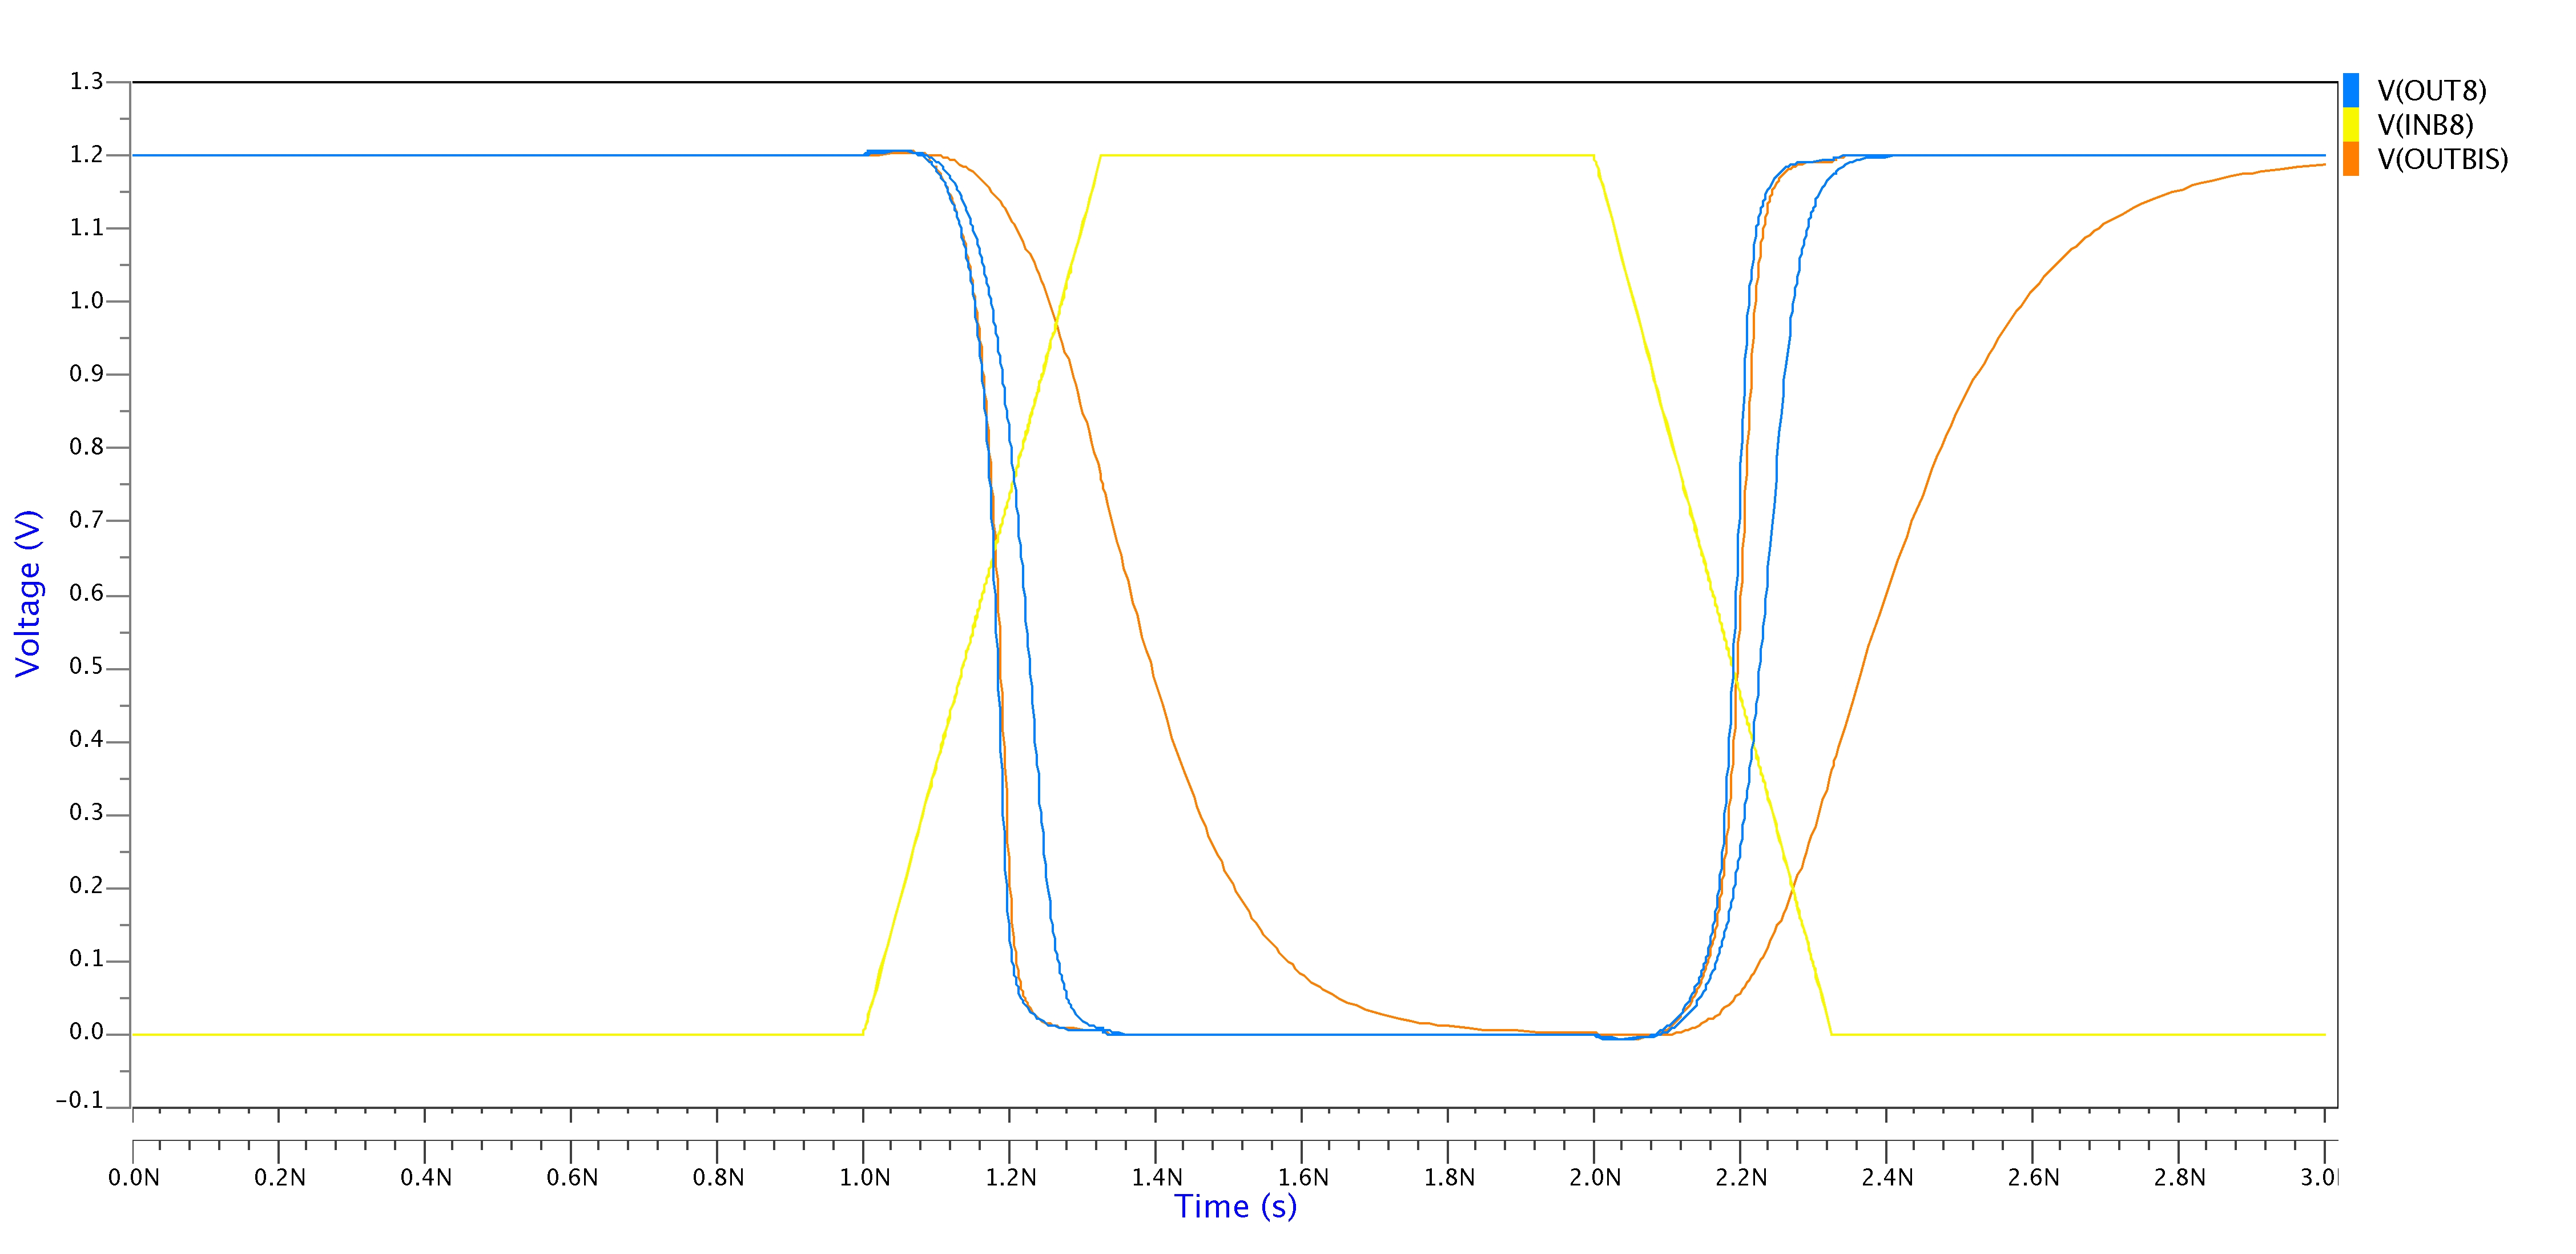
\includegraphics[scale=0.09]{immagini/onde_5_3_voltage1}
	\caption{\textit{Confronto delle tensioni}}
	\label{onde_5_3_voltage1}
\end{figure}
\begin{figure}[!htb]
	\centering
	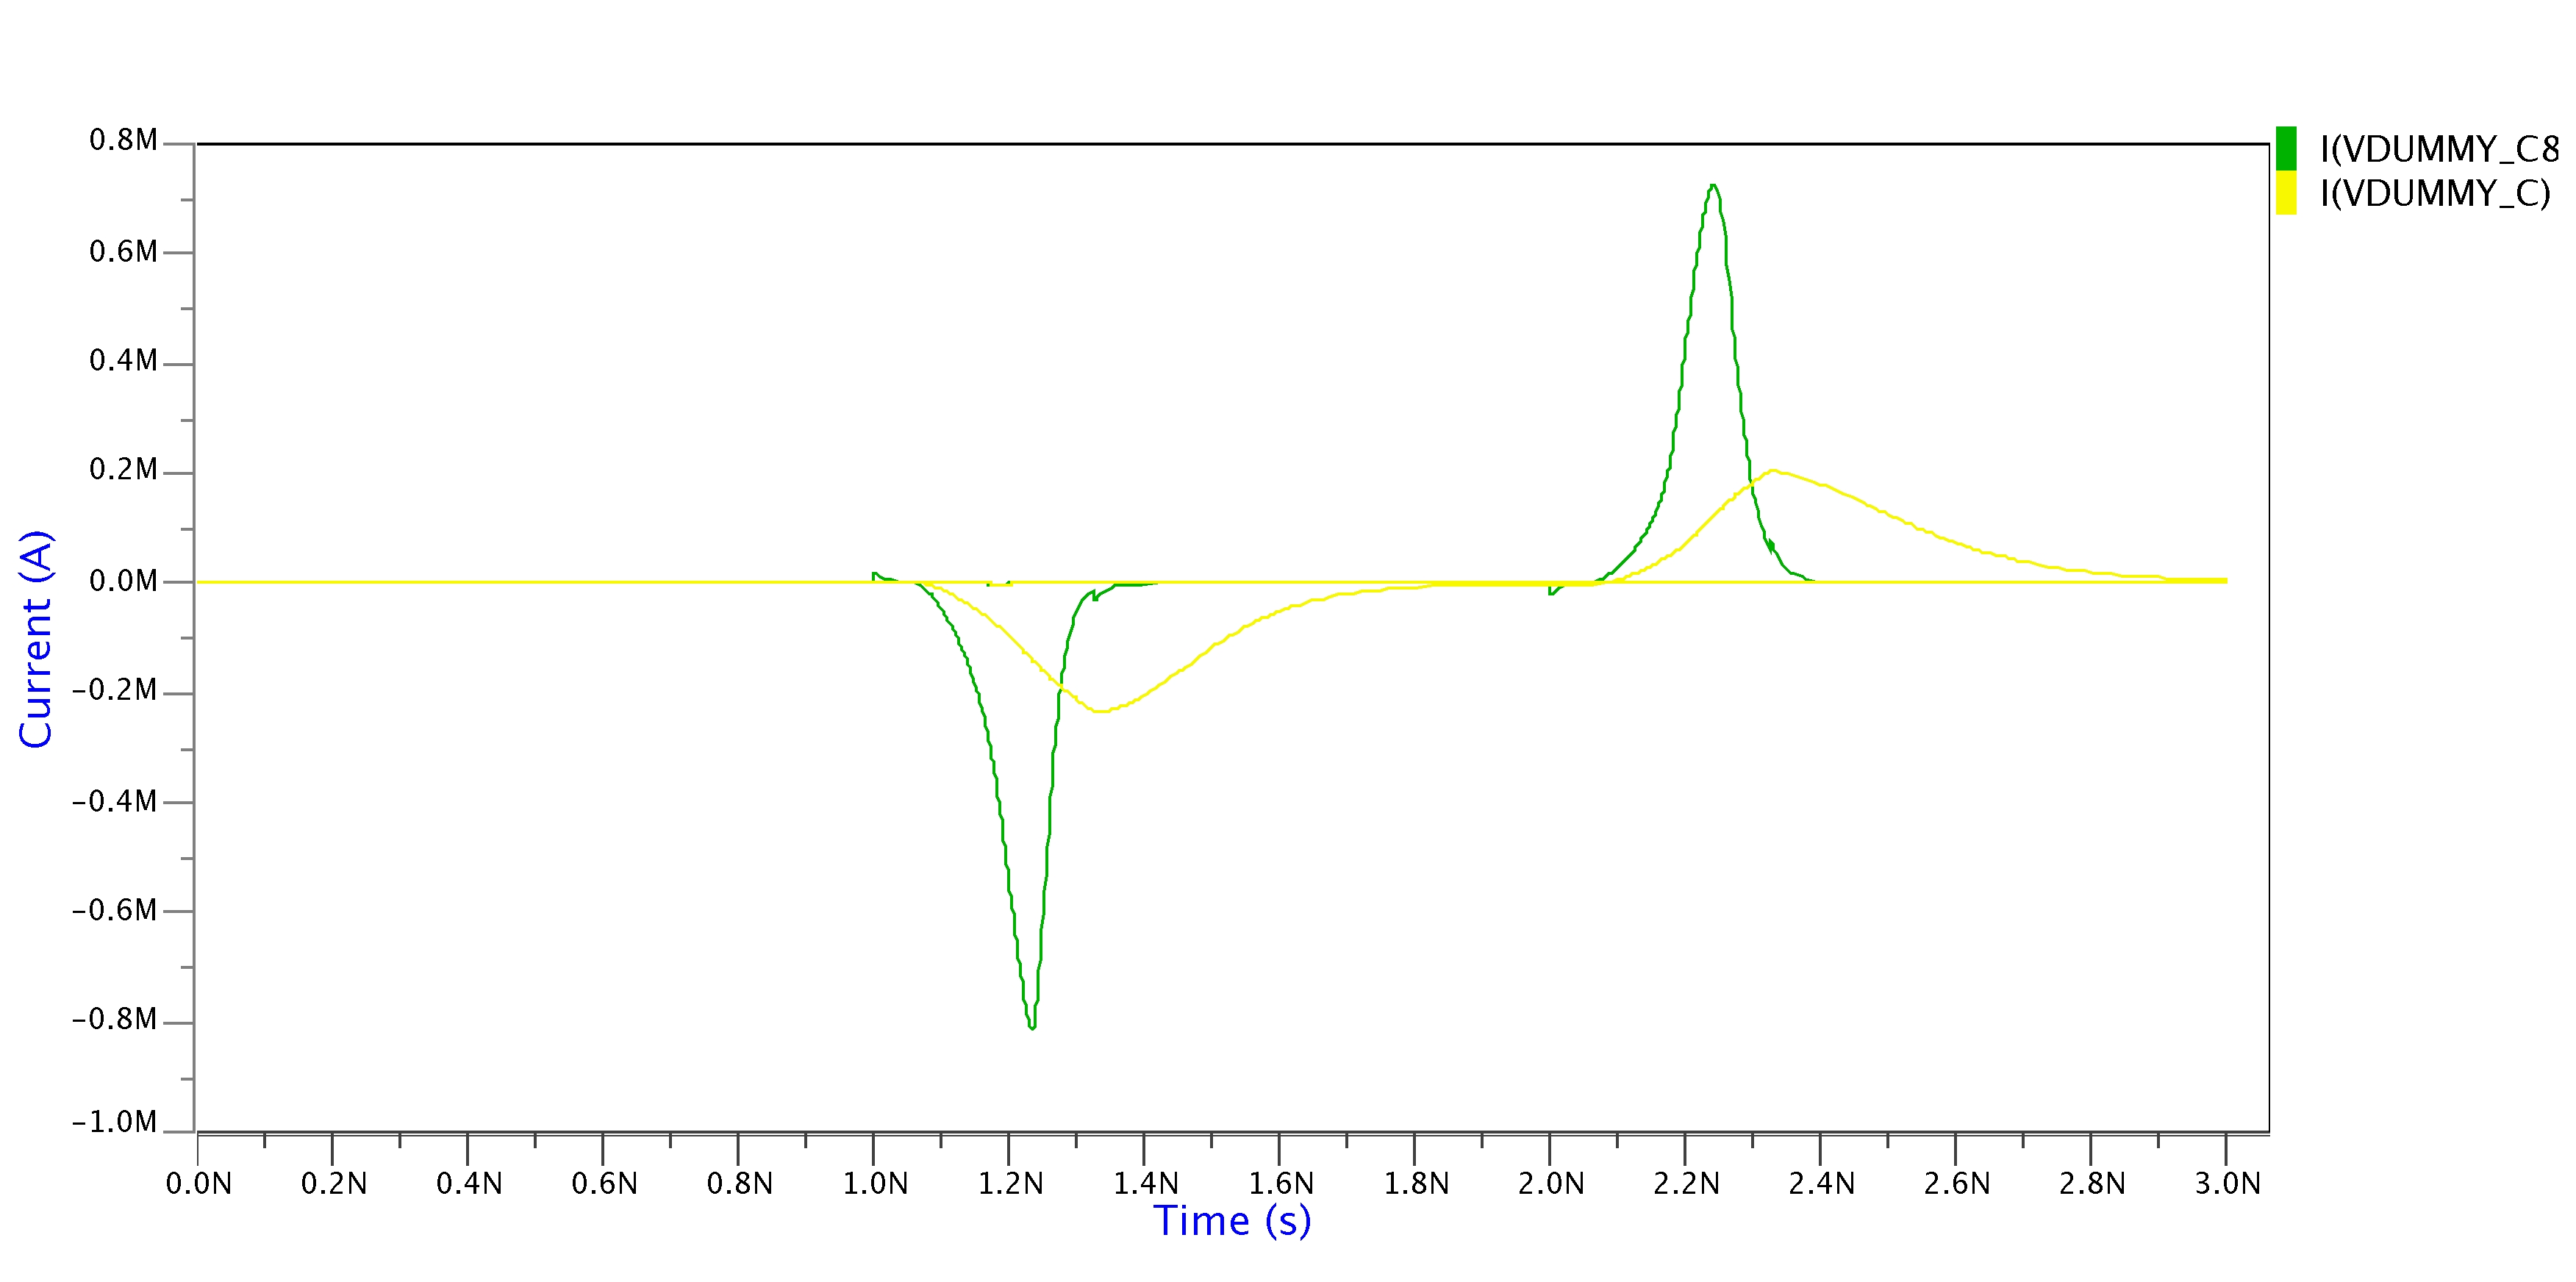
\includegraphics[scale=0.12]{immagini/onde_5_3_current1}
	\caption{\textit{Confronto delle correnti load}}
	\label{onde_5_3_current1}
\end{figure}
\newpage
\begin{figure}[!htb]
	\centering
	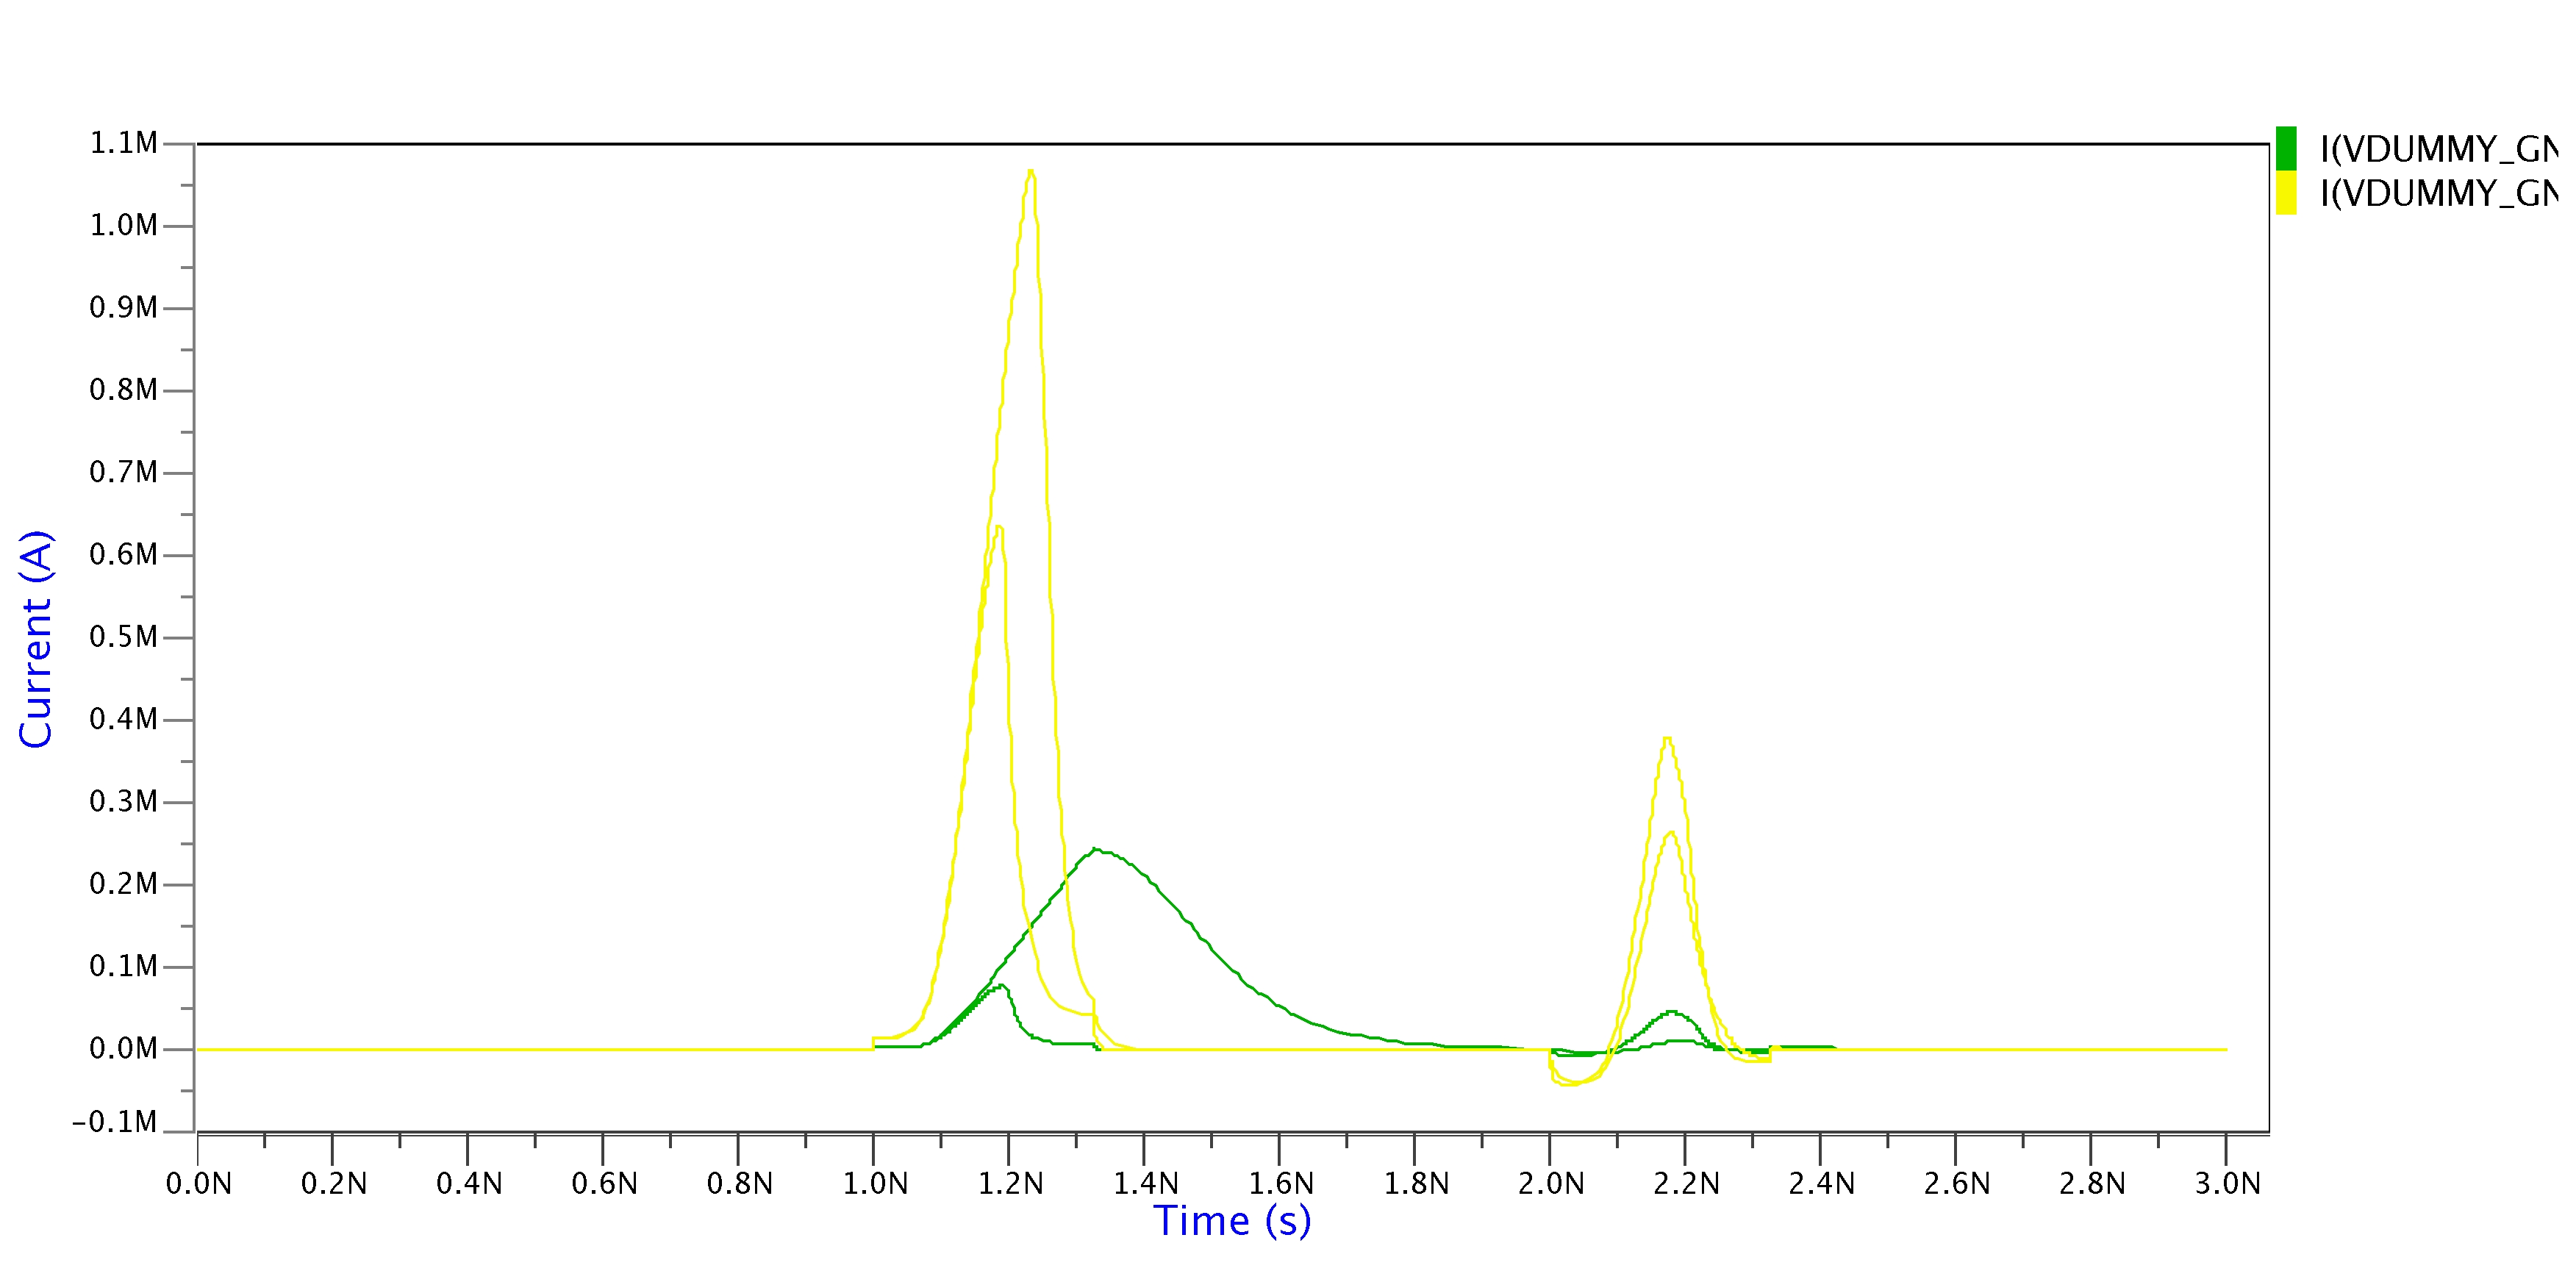
\includegraphics[scale=0.12]{immagini/onde_5_3_current2}
	\caption{\textit{Confronto delle correnti ground}}
	\label{onde_5_3_current2}
\end{figure}
\begin{figure}[!htb]
	\centering
	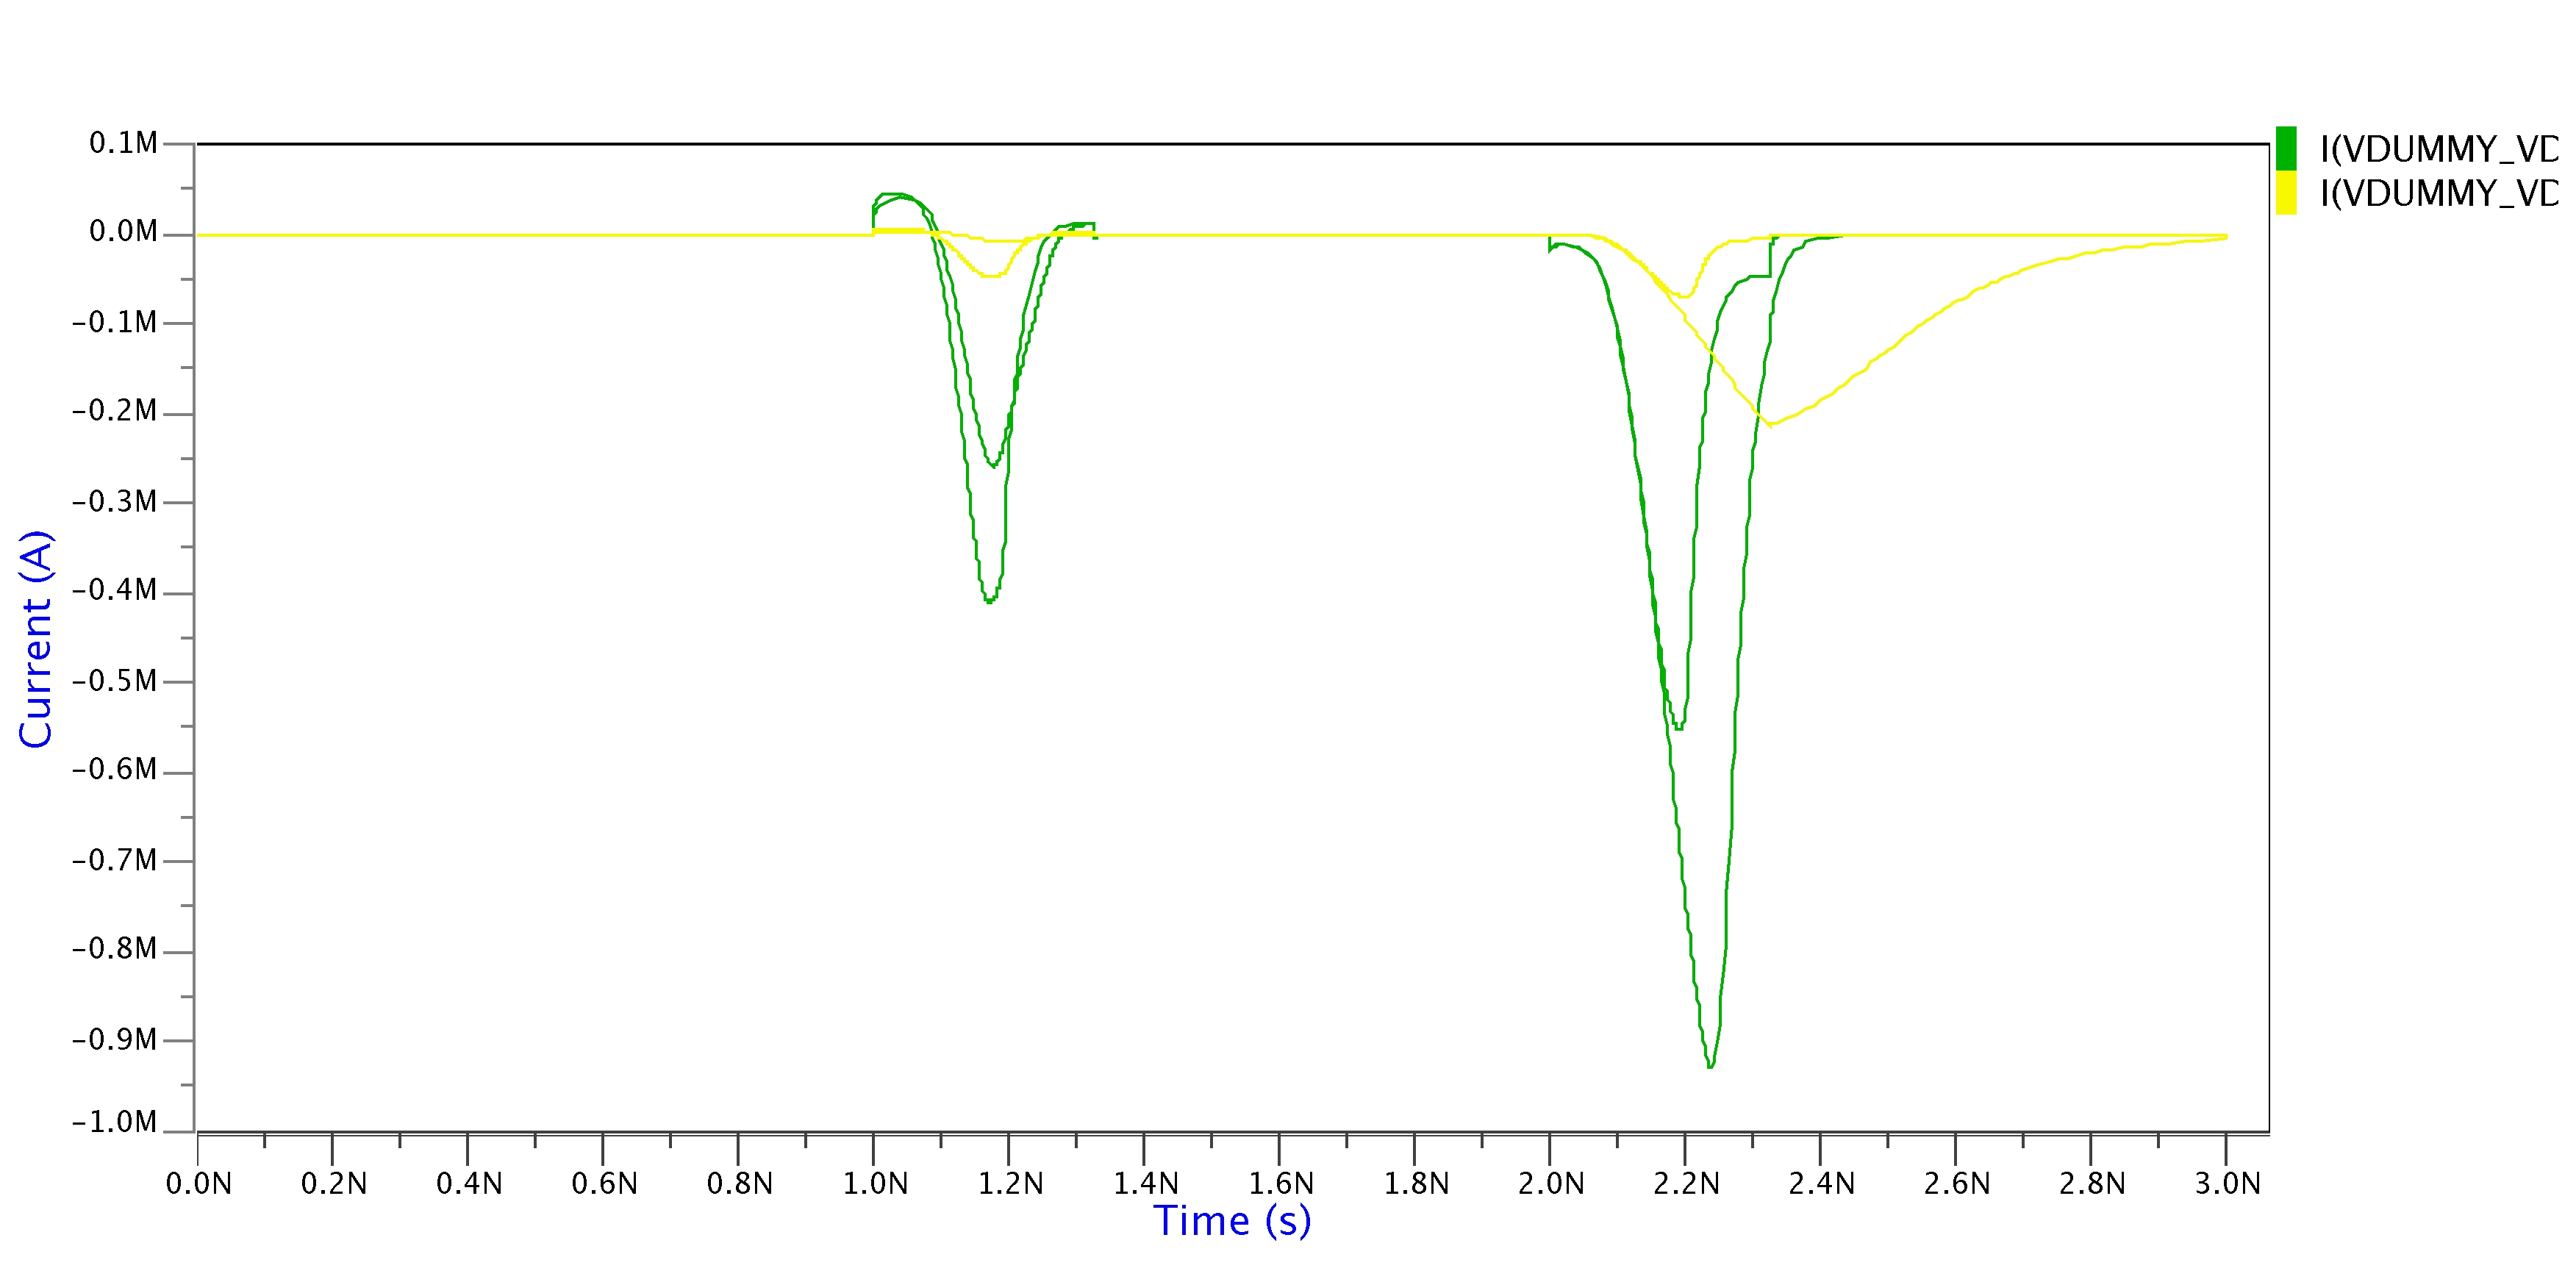
\includegraphics[scale=0.12]{immagini/onde_5_3_current3}
	\caption{\textit{Confronto delle correnti vdd}}
	\label{onde_5_3_current3}
\end{figure}
\newpage
\noindent Infine si riportano nelle Tabelle \ref{Tab5_11} e \ref{Tab5_12} i risultati delle tensioni di soglia, rispettivamente della NAND X1 e della NAND X8, ottenuti attraverso la simulazione dc.
\begin{table}[!h]\footnotesize
	\centering
	\begin{tabular}{|c|c|c|}
		\hline
		\textbf{NAND X1} &&\\
		
		\textbf{Transistor/$C_{Load}$}&0.06 pF & 60 pF\\
		\hline
		\textbf{XMN0.M1} &0.31371&0.31371\\
		
		\textbf{XMN1.M1} &0.27241&0.27241 \\
		
		\textbf{XMP0.M1}&-0.24712&-0.24712 \\
		
		\textbf{XMP1.M1}&-0.24712&-0.247122\\
		
		\hline
	\end{tabular}
	\caption{\textit{Tensioni di soglia}}
	\label{Tab5_11}
\end{table}
\begin{table}[!h]\footnotesize
	\centering
	\begin{tabular}{|c|c|c|}
		\hline
		\textbf{NAND X8} &&\\
		
		\textbf{Transistor/$C_{Load}$}&0.06 pF & 60 pF\\
		\hline
		\textbf{XMN0.M1} &0.31893&0.31893\\
		
		\textbf{XMN1.M1} &0.27763&0.27763 \\
		
		\textbf{XMN2.M1} &0.31893&0.31893\\
		
		\textbf{XMN3.M1} &0.27763&0.27763 \\
		\textbf{XMN4.M1} &0.27763&0.27763 \\
		\textbf{XMN5.M1} &0.31893&0.31893\\
		
		\textbf{XMN6.M1} &0.27763&0.27763 \\
		\textbf{XMN7.M1} &0.31893&0.31893\\
		
		\textbf{XMP0.M1}&-0.24712&-0.24712 \\
		
		\textbf{XMP1.M1}&-0.24712&-0.24712\\
		\textbf{XMP6.M1}&-0.24712&-0.24712 \\
		
		\textbf{XMP7.M1}&-0.24712&-0.24712\\
		
		\hline
	\end{tabular}
	\caption{\textit{Tensioni di soglia}}
	\label{Tab5_12}
\end{table}

\section{Comparing high speed and low leakage optimization}
Viene ora richiesto di fare le medesime analisi svolte nei punti precedenti, ma utilizzando delle tipologie di gate ottimizzati per una bassa corrente sottosoglia. I modelli utilizzati sono precisamente: \textbf{ND2LL} e \textbf{ND2LLX8}. \\
I dati raccolti dalla simulazione ELDO sono riportati:
\begin{itemize}
	\item per quanto riguarda il transistore X1, nella Tabella \ref{Tab5_13} per i tempi, mentre nella Tabella \ref{Tab5_14} per le correnti.
	\item per quanto riguarda il transistore X8, nella Tabella \ref{Tab5_15} per i tempi, mentre nella Tabella \ref{Tab5_16} per le correnti.
\end{itemize}
\begin{table}[!h]\footnotesize
	\centering
	\begin{tabular}{|c|c|c|}
		\hline
		\textbf{NAND LL X1} & &\\
		\textbf{$C_{Load}$} & \textbf{0.06 fF} & \textbf{60 fF}\\
		\hline
		$t_{rise}$ &71.556 ps&592.23 ps  \\
		
		$t_{fall}$ &63.464 ps &406.23 ps  \\
		
		$t_{pdHL}$&31.612 ps &257.67 ps  \\
		
		$t_{pdLH}$ &52.657 ps&331.22 ps  \\
		
		\hline
	\end{tabular}
	\caption{\textit{Risultati tempi simulazione ELDO, NAND LL X1}}
	\label{Tab5_13}
\end{table}
\begin{table}[!h]\footnotesize
	\centering
	\begin{tabular}{|c|c|c|}
		\hline
		\textbf{NAND LL X1} & &\\
		\textbf{$C_{Load}$} & \textbf{0.06 fF} & \textbf{60 fF}\\
		\hline
		$I_{GND, f}^{max}$ &404.32$\mu$A &867.10 $\mu$A\\
		
		$I_{Vdd, r}^{max}$ &-303.01$\mu$A &-683.65 $\mu$A \\
		
		$I_{GND, r}^{max}$&132.79 $\mu$A &68.306 $\mu$A\\
		
		$I_{Vdd, f}^{max}$&-165.52 $\mu$A&-70.310 $\mu$A \\
		
		$I_{Load, f}^{max}$ &3.2194 nA &3.3727 nA \\
		
		$I_{Load, r}^{max}$ &-2.4740 nA &-3.2278 nA  \\
		\hline
	\end{tabular}
	\caption{\textit{Risultati delle correnti simulazione ELDO, NAND LL X1}}
	\label{Tab5_14}
\end{table}
\begin{table}[!h]\footnotesize
	\centering
	\begin{tabular}{|c|c|c|}
		\hline
		\textbf{NAND LL X8} & &\\
		\textbf{$C_{Load}$} & \textbf{0.06 fF} & \textbf{60 fF}\\
		\hline
		$t_{rise}$ &63.480 ps&137.67 ps  \\
		
		$t_{fall}$ &57.371 ps &112.39 ps  \\
		
		$t_{pdHL}$&26.768 ps &78.324 ps  \\
		
		$t_{pdLH}$ &44.524 ps&102.77 ps  \\
		\hline
	\end{tabular}
	\caption{\textit{Risultati tempi simulazione ELDO, NAND LL X8}}
	\label{Tab5_15}
\end{table}
\begin{table}[!h]\footnotesize
	\centering
	\begin{tabular}{|c|c|c|}
		\hline
		\textbf{NAND LL X8} & &\\
		\textbf{$C_{Load}$} & \textbf{0.06 fF} & \textbf{60 fF}\\
		\hline
		$I_{GND, f}^{max}$ &51.878 $\mu$A &194.22 $\mu$A\\
		
		$I_{Vdd, r}^{max}$ &-42.315$\mu$A &-151.76 $\mu$A \\
		
		$I_{GND, r}^{max}$&16.961 $\mu$A &3.6258 $\mu$A\\
		
		$I_{Vdd, f}^{max}$&-19.758 $\mu$A&-2.4801 $\mu$A \\
		
		$I_{Load, f}^{max}$ &0.39863 nA &1923.7 nA \\
		
		$I_{Load, r}^{max}$ &-0.37117 nA &-36.882 nA  \\
		\hline
	\end{tabular}
	\caption{\textit{Risultati delle correnti simulazione ELDO, NAND LL X1}}
	\label{Tab5_16}
\end{table}
Si può ben notare come, tutti i tempi si siano dilatati per le porte \textit{Low Leakage} rispetto a quelle \textit{High Speed}. Si può analizzare l'incremento percentuale del caso LL rispetto al caso HS nella Tabella \ref{Tab5_17} per il gate X1 e nella Tabella \ref{Tab5_18} per il gate X8.
\begin{table}[!h]\footnotesize
	\centering
	\begin{tabular}{|c|c|c|}
		\hline
		\textbf{Confronto LL-HS} & &\\
		\textbf{NAND X1} & &\\
		\textbf{$C_{Load}$} & \textbf{0.06 fF} & \textbf{60 fF}\\
		\hline
		$t_{rise}$ &5.71\% &39.33\%  \\
		
		$t_{fall}$ &\% & 18.86\%  \\
		
		$t_{pdHL}$&51.1\% & 26.49\%  \\
		
		$t_{pdLH}$&37.27\%& 39.98\% \\
		\hline
	\end{tabular}
	\caption{\textit{Aumento percentuale dei tempi LL/HS NAND X1}}
	\label{Tab5_17}
\end{table}
\begin{table}[!h]\footnotesize
	\centering
	\begin{tabular}{|c|c|c|}
		\hline
		\textbf{Confronto LL-HS} & &\\
		\textbf{NAND X8} & &\\
		\textbf{$C_{Load}$} & \textbf{0.06 fF} & \textbf{60 fF}\\
		\hline
		$t_{rise}$ &16.43\% &21.76\%  \\
		
		$t_{fall}$ &\% & 5.16\%  \\
		
		$t_{pdHL}$&53.27\% &36.36\%  \\
		
		$t_{pdLH}$&41.99\%& 42.23\% \\
		\hline
	\end{tabular}
	\caption{\textit{Aumento percentuale dei tempi LL/HS NAND X8}}
	\label{Tab5_18}
\end{table}
\\
Al contrario, si può ben notare come le varie correnti si riducano dal caso LL rispetto al caso HS, arrivando anche a diminuire di un ordine di grandezza. In Tabella \ref{Tab5_19} e in Tabella \ref{Tab5_20} si può notare quanto valga la riduzione percentuale della corrente dal caso HS al caso LL, rispettivamente per il gate X1 e il gate X8.
\begin{table}[!h]\footnotesize
	\centering
	\begin{tabular}{|c|c|c|}
		\hline
		\textbf{NAND LL X1} & &\\
		\textbf{$C_{Load}$} & \textbf{0.06 fF} & \textbf{60 fF}\\
		\hline
		$I_{GND, f}^{max}$ &32.78\%  &20.88\% \\
		
		$I_{Vdd, r}^{max}$ &39.99\% &29.32\% \\
		
		$I_{GND, r}^{max}$&62.85\% &66.93\%\\
		
		$I_{Vdd, f}^{max}$&58.52\% &73.83\% \\
		
		$I_{Load, f}^{max}$ &95.19\% &?????\\
		
		$I_{Load, r}^{max}$ &93.44\% &????  \\
		\hline
	\end{tabular}
	\caption{\textit{Riduzione percentuale delle correnti NAND X1}}
	\label{Tab5_19}
\end{table}
\begin{table}[!h]\footnotesize
	\centering
	\begin{tabular}{|c|c|c|}
		\hline
		\textbf{NAND LL X8} & &\\
		\textbf{$C_{Load}$} & \textbf{0.06 fF} & \textbf{60 fF}\\
		\hline
		$I_{GND, f}^{max}$ &32.78\%  &20.88\% \\
		
		$I_{Vdd, r}^{max}$ &39.99\% &29.32\% \\
		
		$I_{GND, r}^{max}$&62.85\% &66.93\%\\
		
		$I_{Vdd, f}^{max}$&58.52\% &73.83\% \\
		
		$I_{Load, f}^{max}$ &95.19\% &-\\
		
		$I_{Load, r}^{max}$ &93.44\% &-\\
		\hline
	\end{tabular}
	\caption{\textit{Riduzione percentuale delle correnti NAND X8}}
	\label{Tab5_20}
\end{table}
\newpage
\noindent In seguito, nelle Tabelle \ref{Tab5_21} e \ref{Tab5_22}, sono riportati rispettivamente i valori delle Tensioni di Soglia dei gate \textit{Low Leakage} rispettivamente nel caso del gate X1 ed il gate X8. Si può notare come i valori siano superiori rispetto a quelli del caso \textit{High Speed}: questo fenomeno è assolutamente concorde con quanto appreso in teoria, in quanto un transistor a basso leakage deve avere delle tensioni di soglia più elevate.
\begin{table}[!h]\footnotesize
	\centering
	\begin{tabular}{|c|c|c|}
		\hline
		\textbf{NAND X1} &&\\
		\textbf{Transistor/$C_{Load}$}&0.06 pF & 60 pF\\
		\hline
		\textbf{XMN0.M1} &0.41333&0.41333\\
		\textbf{XMN1.M1} &0.38062&0.38062 \\
		\textbf{XMP0.M1}&-0.36712&-0.36712 \\
		\textbf{XMP1.M1}&-0.36712&-0.36712\\
		\hline
	\end{tabular}
	\caption{\textit{Tensioni di soglia}}
	\label{Tab5_21}
\end{table}
\begin{table}[!h]\footnotesize
	\centering
	\begin{tabular}{|c|c|c|}
		\hline
		\textbf{NAND X8} &&\\
		
		\textbf{Transistor/$C_{Load}$}&0.06 pF & 60 pF\\
		\hline
		\textbf{XMN0.M1} &0.41333&0.41333\\	
		\textbf{XMN1.M1} &0.38062&0.38062 \\
		\textbf{XMN2.M1} &0.41333&0.41333\\
		\textbf{XMN3.M1} &0.38062&0.38062 \\
		\textbf{XMN4.M1} &0.38062&0.38062 \\
		\textbf{XMN5.M1} &0.41333&0.41333\\
		\textbf{XMN6.M1} &0.38062&0.38062 \\
		\textbf{XMN7.M1} &0.41333&0.41333\\
		\textbf{XMP0.M1}&-&- \\
		\textbf{XMP1.M1}&-&-\\
		\textbf{XMP6.M1}&-0.36764&-0.36764 \\
		\textbf{XMP7.M1}&-0.36764&-0.36764\\
		
		\hline
	\end{tabular}
	\caption{\textit{Tensioni di soglia}}
	\label{Tab5_22}
\end{table}
\\
Vengono confrontate, tramite \textit{ezwave}, le tensioni e le correnti nei casi \textit{High Speed} e \textit{Low Leakage}. Tutti i grafici risultanti sono riportati nelle Figure \ref{onde_5_4_voltage1},\ref{onde_5_4_voltage2},\ref{onde_5_4_current1},\ref{onde_5_4_current2} ,\ref{onde_5_4_current3}.
\begin{figure}[!htb]
	\centering
	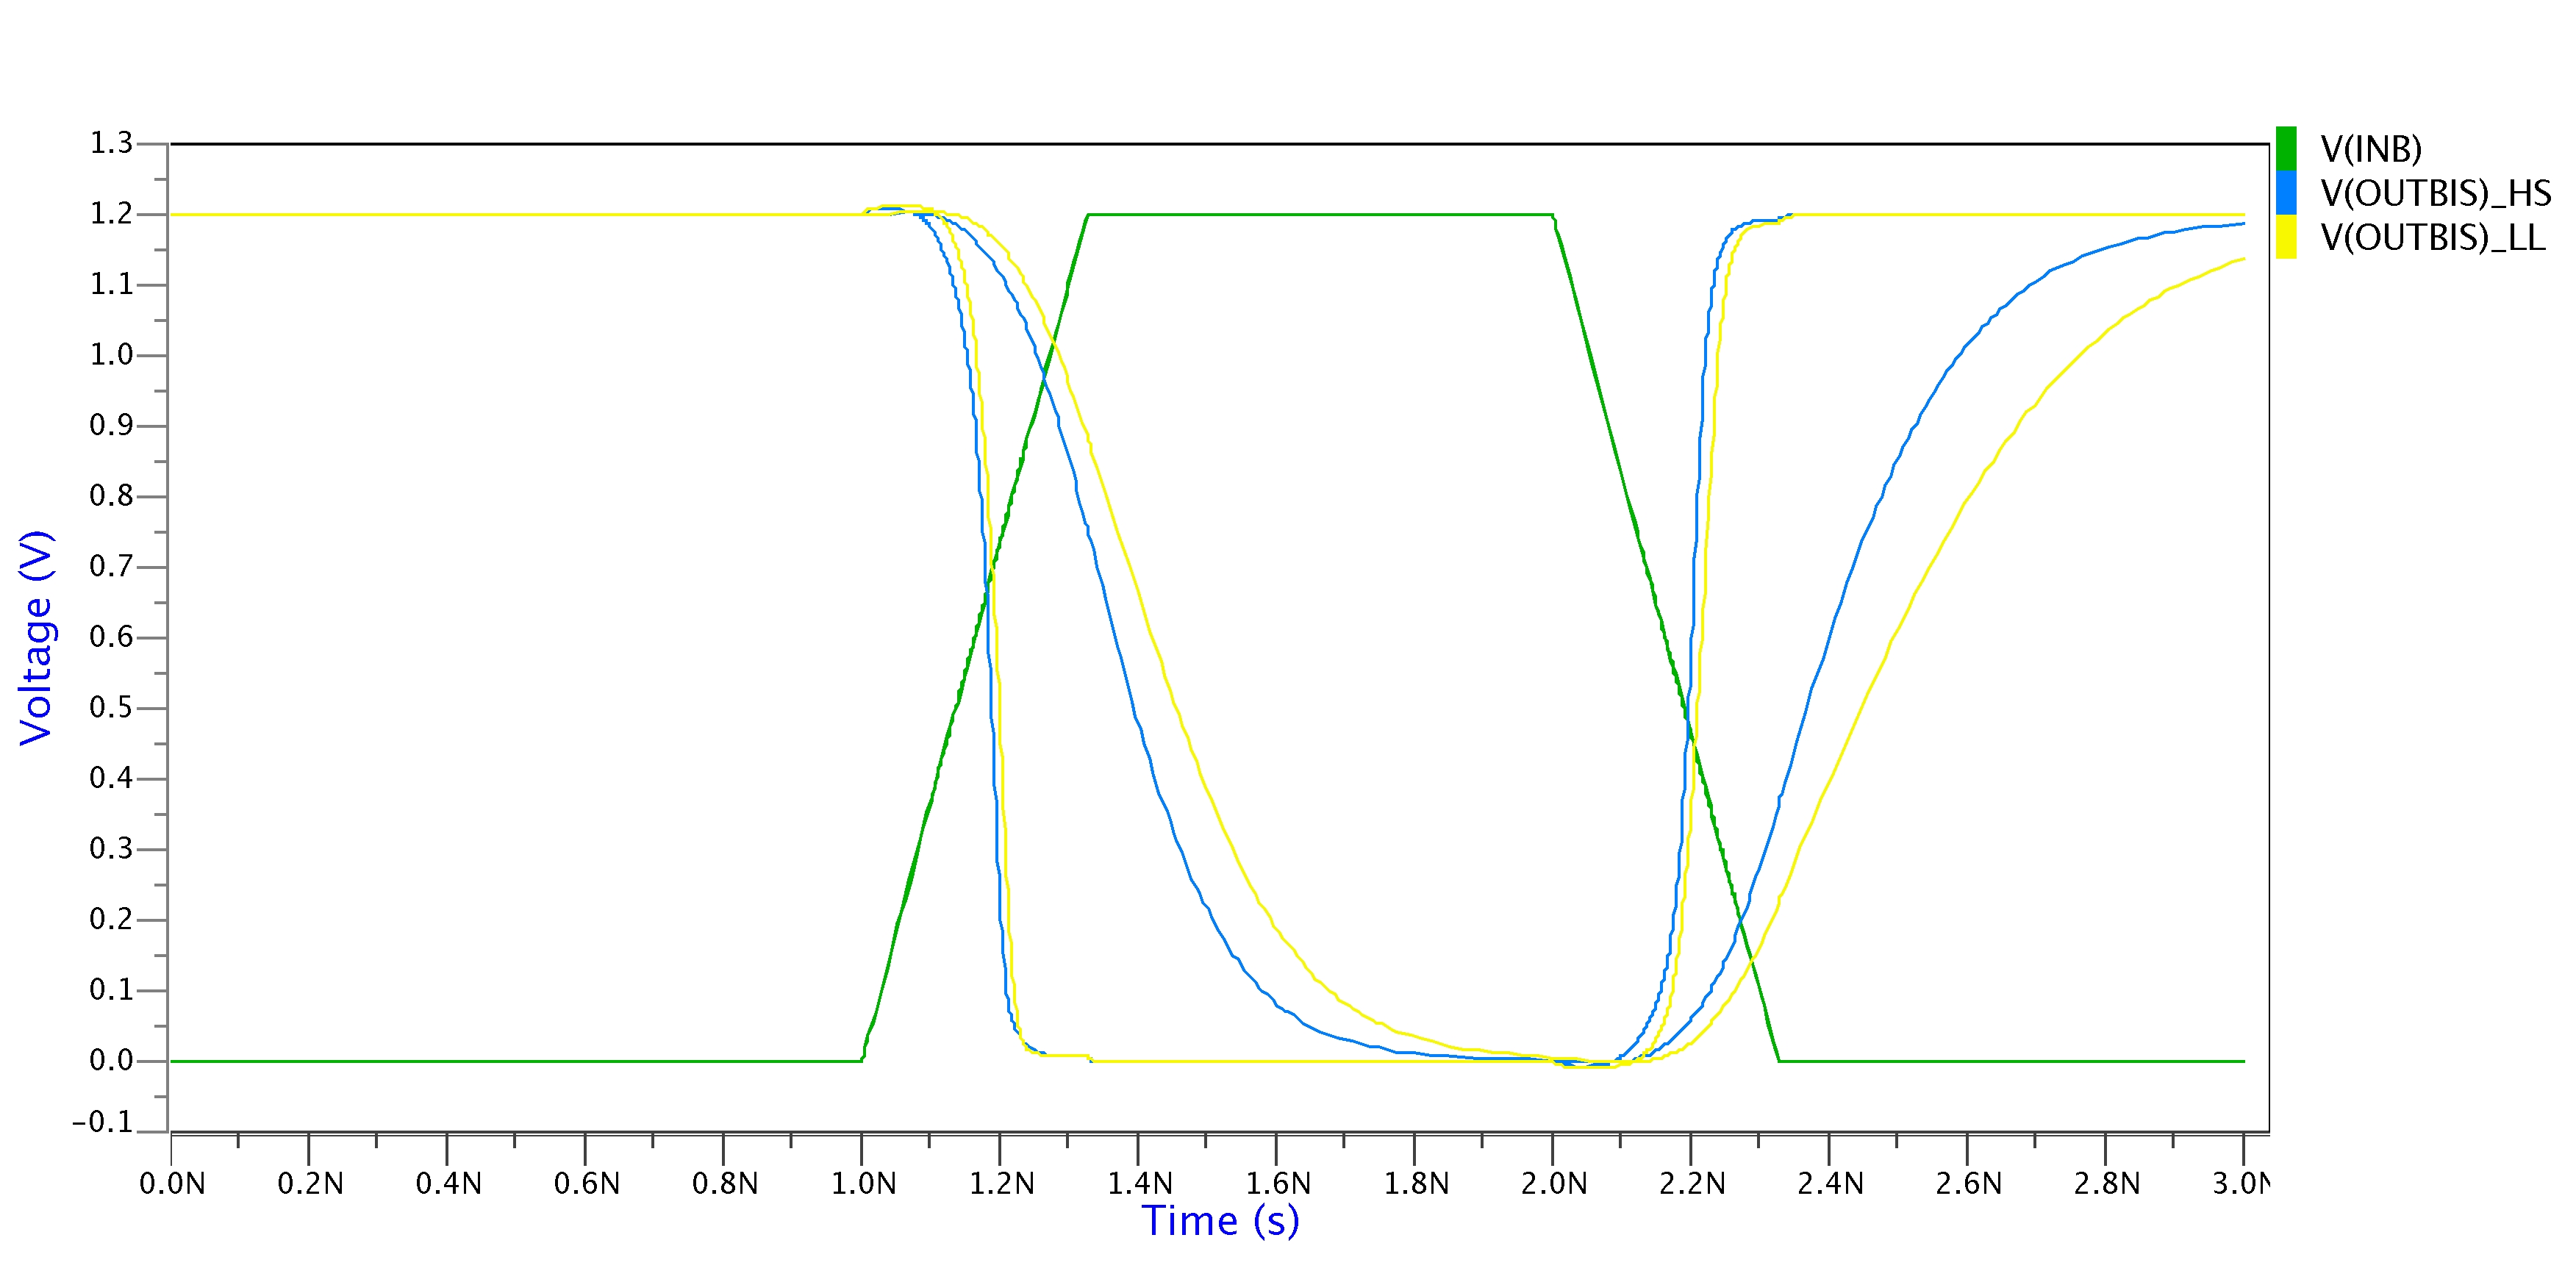
\includegraphics[scale=0.1]{immagini/onde_5_4_voltage1}
	\caption{\textit{Schema circuitale porta NAND}}
	\label{onde_5_4_voltage1}
\end{figure}
\begin{figure}[!htb]
	\centering
	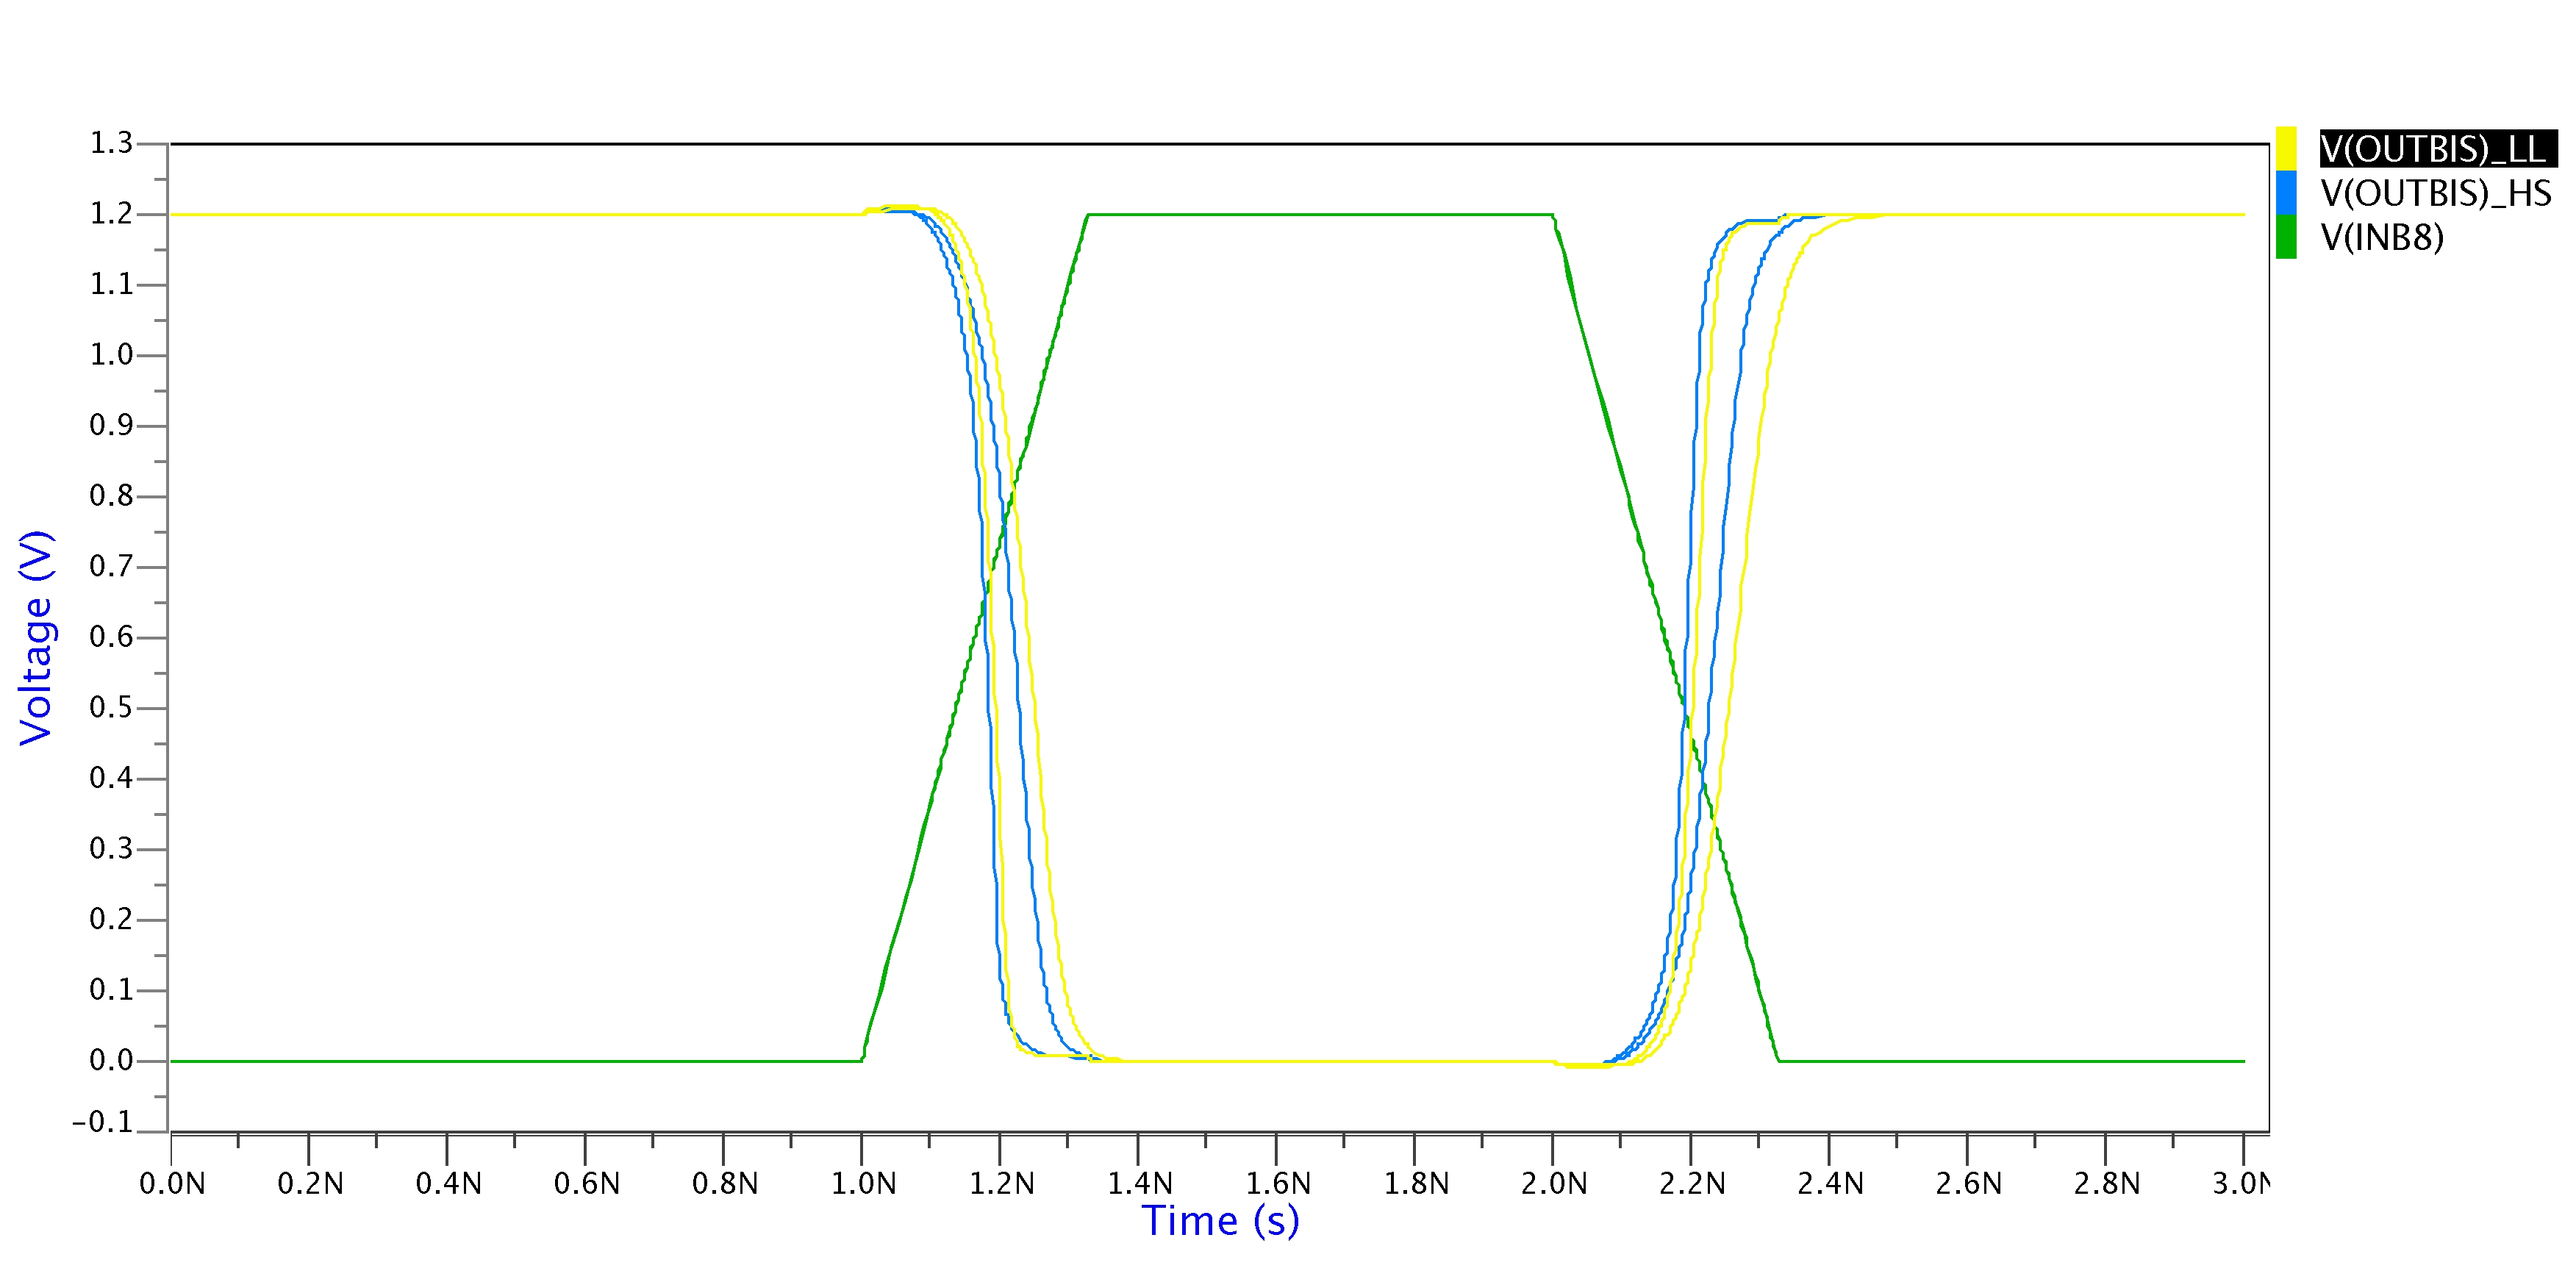
\includegraphics[scale=0.1]{immagini/onde_5_4_voltage2}
	\caption{\textit{Schema circuitale porta NAND}}
	\label{onde_5_4_voltage2}
\end{figure}
\newpage
\begin{figure}[!htb]
	\centering
	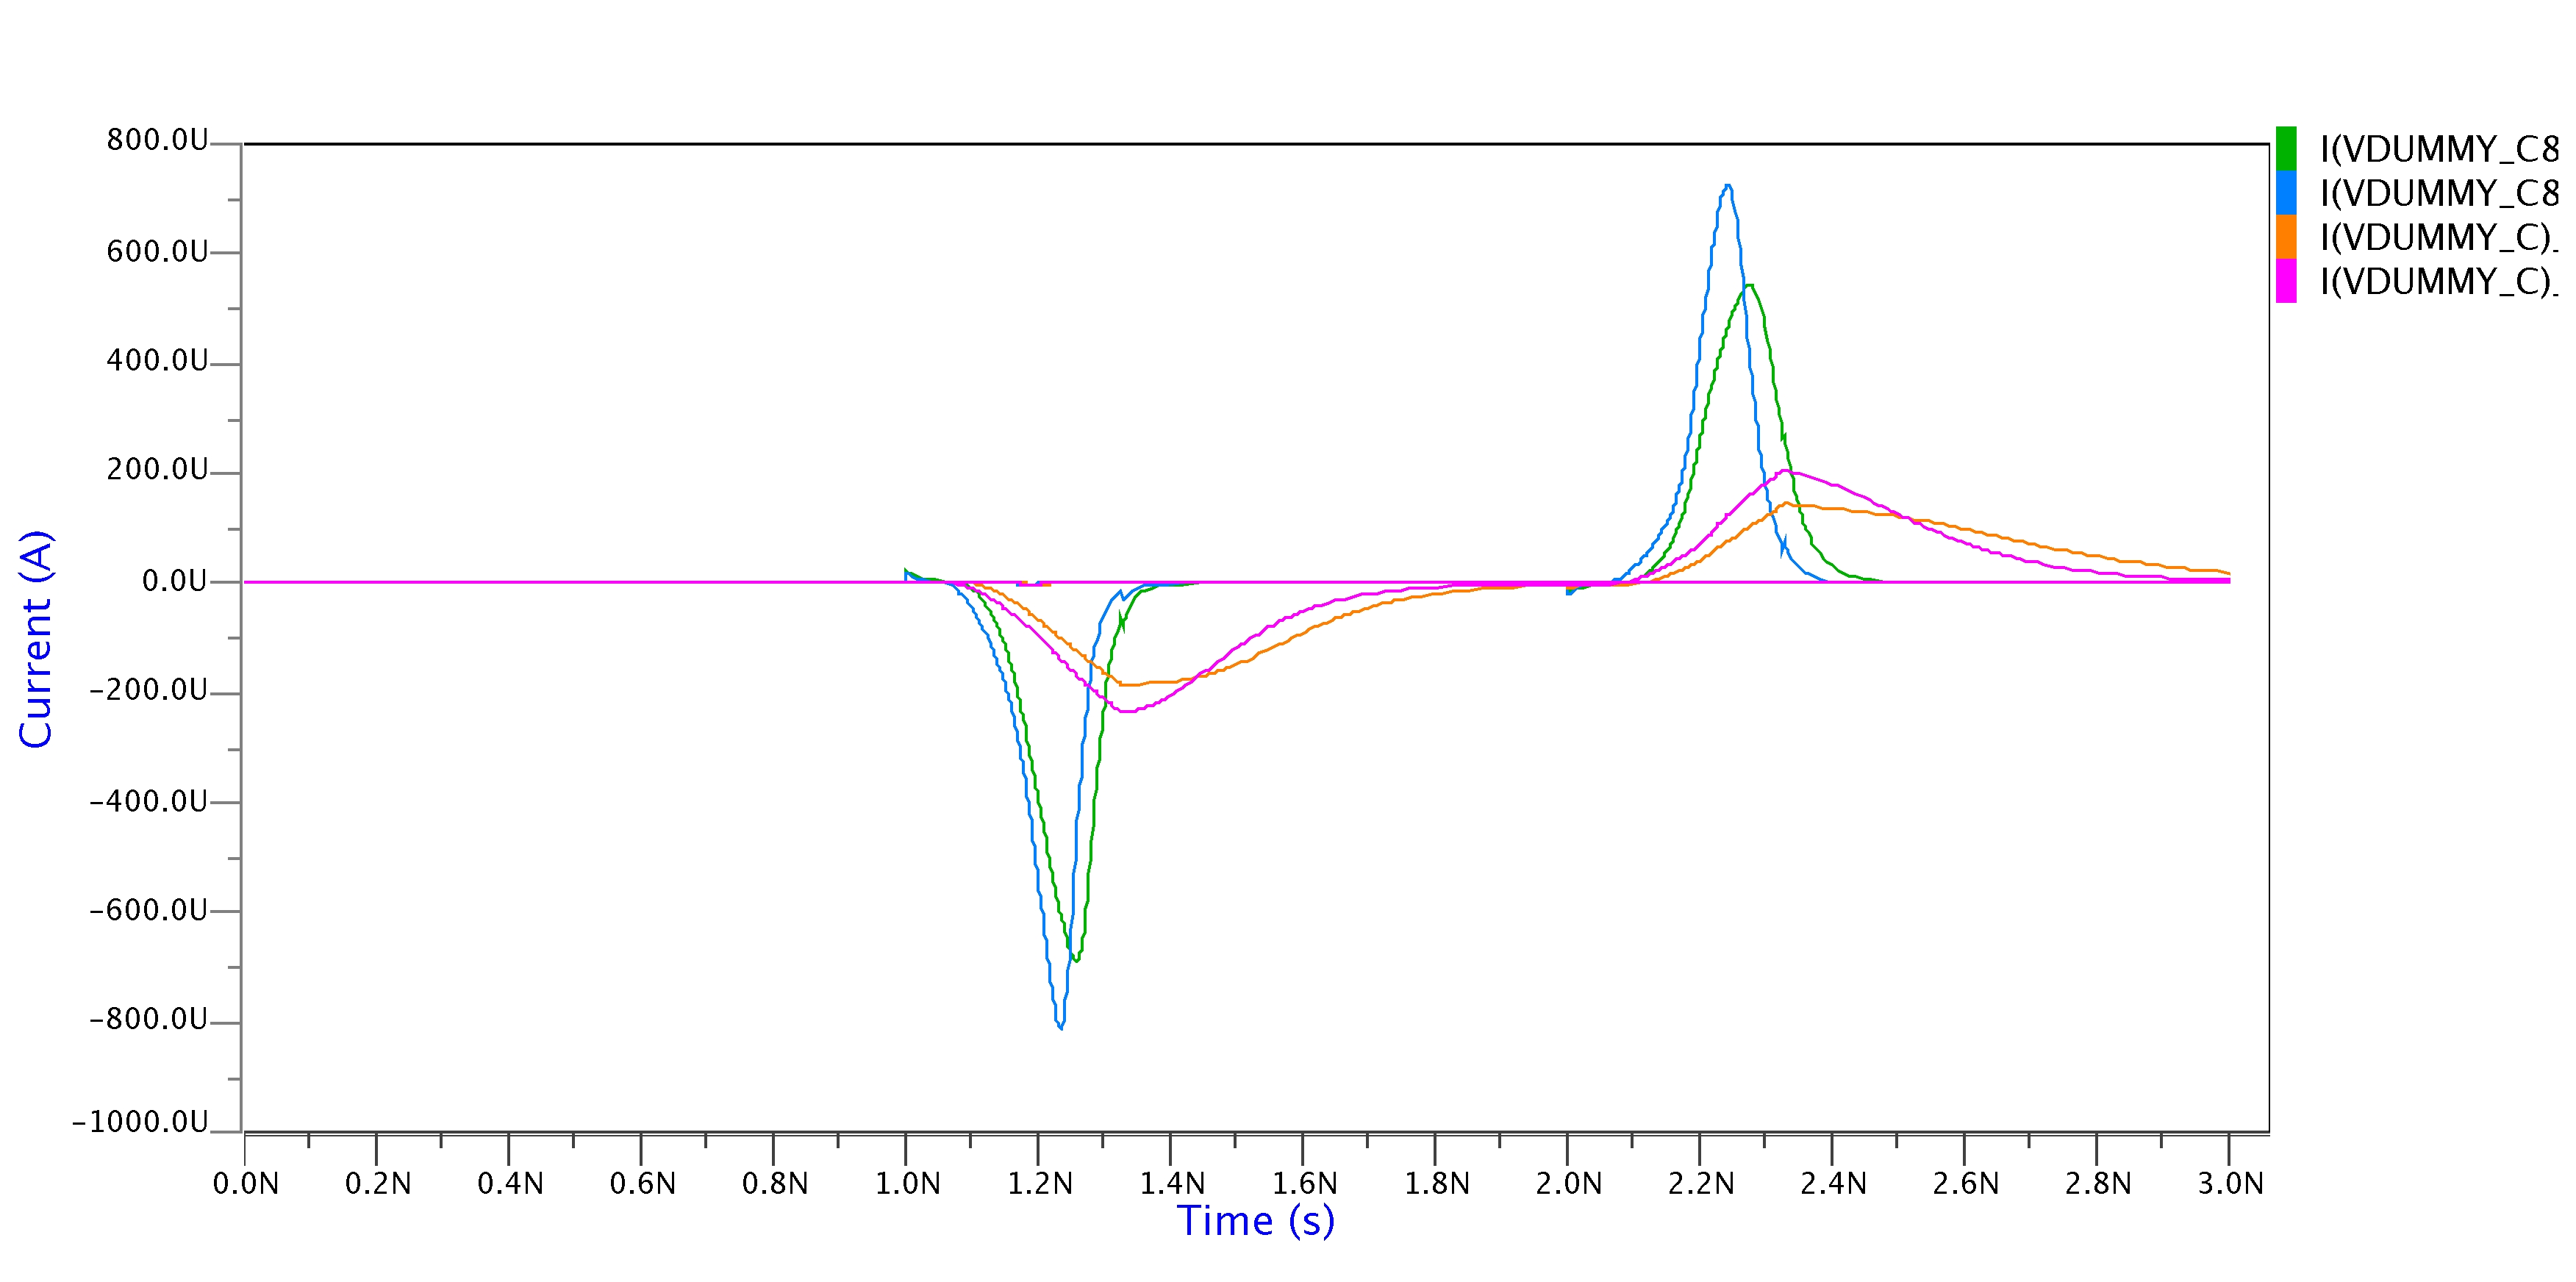
\includegraphics[scale=0.12]{immagini/onde_5_4_current1}
	\caption{\textit{Schema circuitale porta NAND}}
	\label{onde_5_4_current1}
\end{figure}
\begin{figure}[!htb]
	\centering
	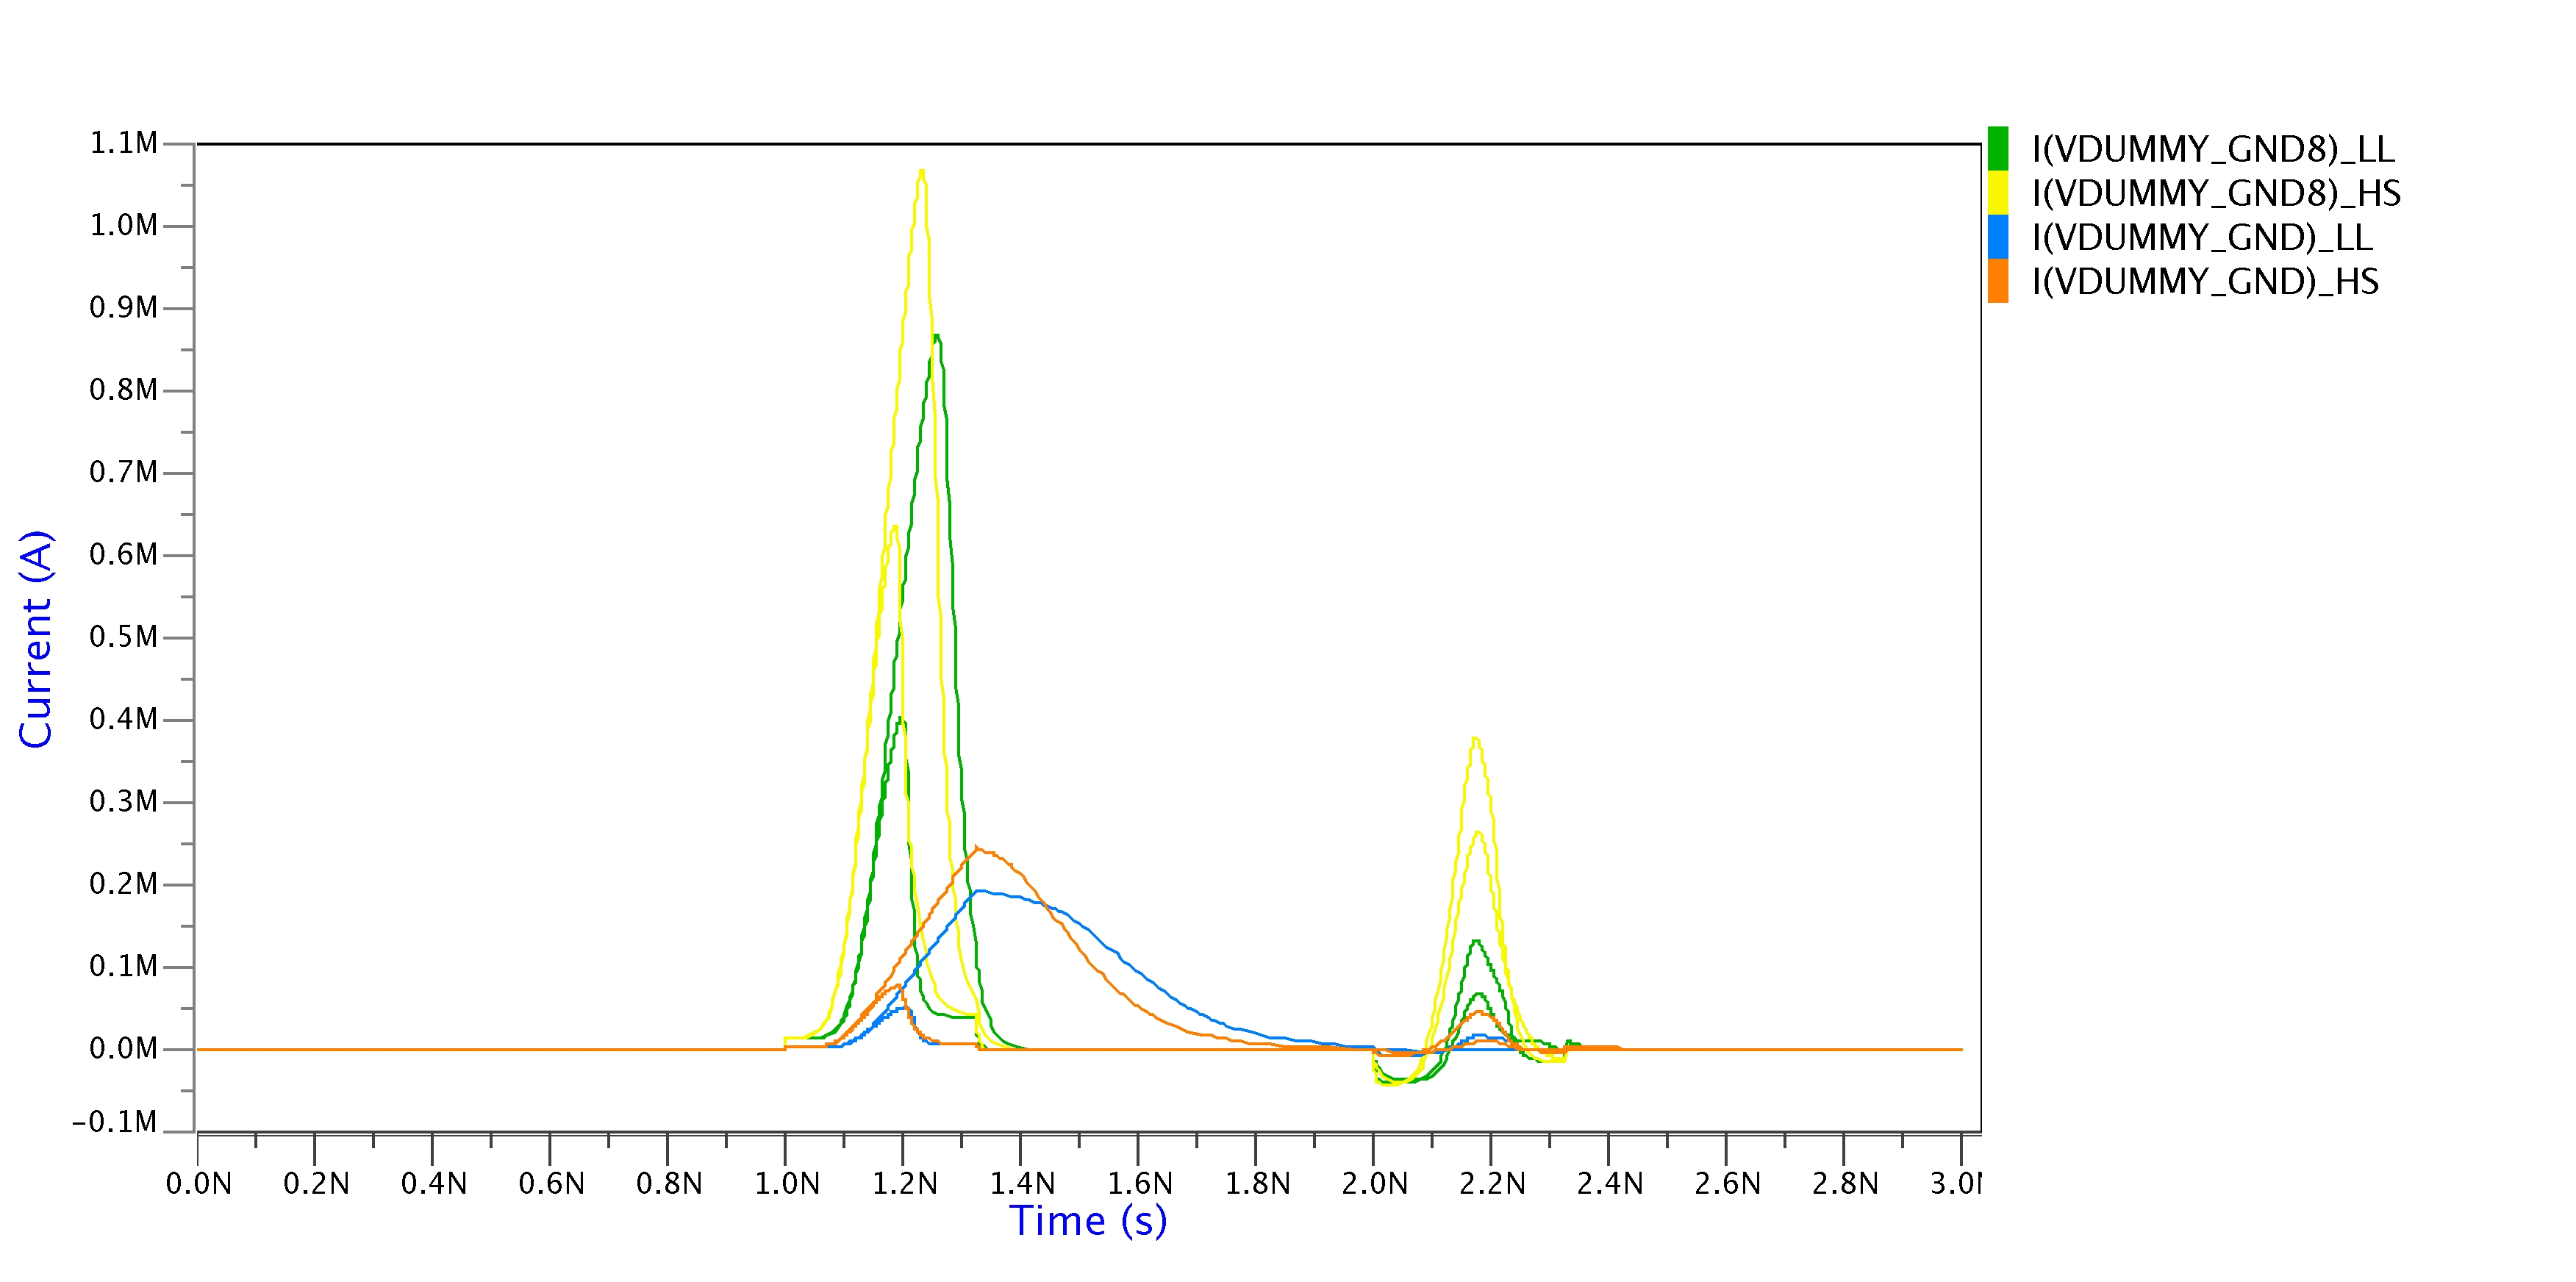
\includegraphics[scale=0.12]{immagini/onde_5_4_current2}
	\caption{\textit{Schema circuitale porta NAND}}
	\label{onde_5_4_current2}
\end{figure}
\newpage
\begin{figure}[!htb]
	\centering
	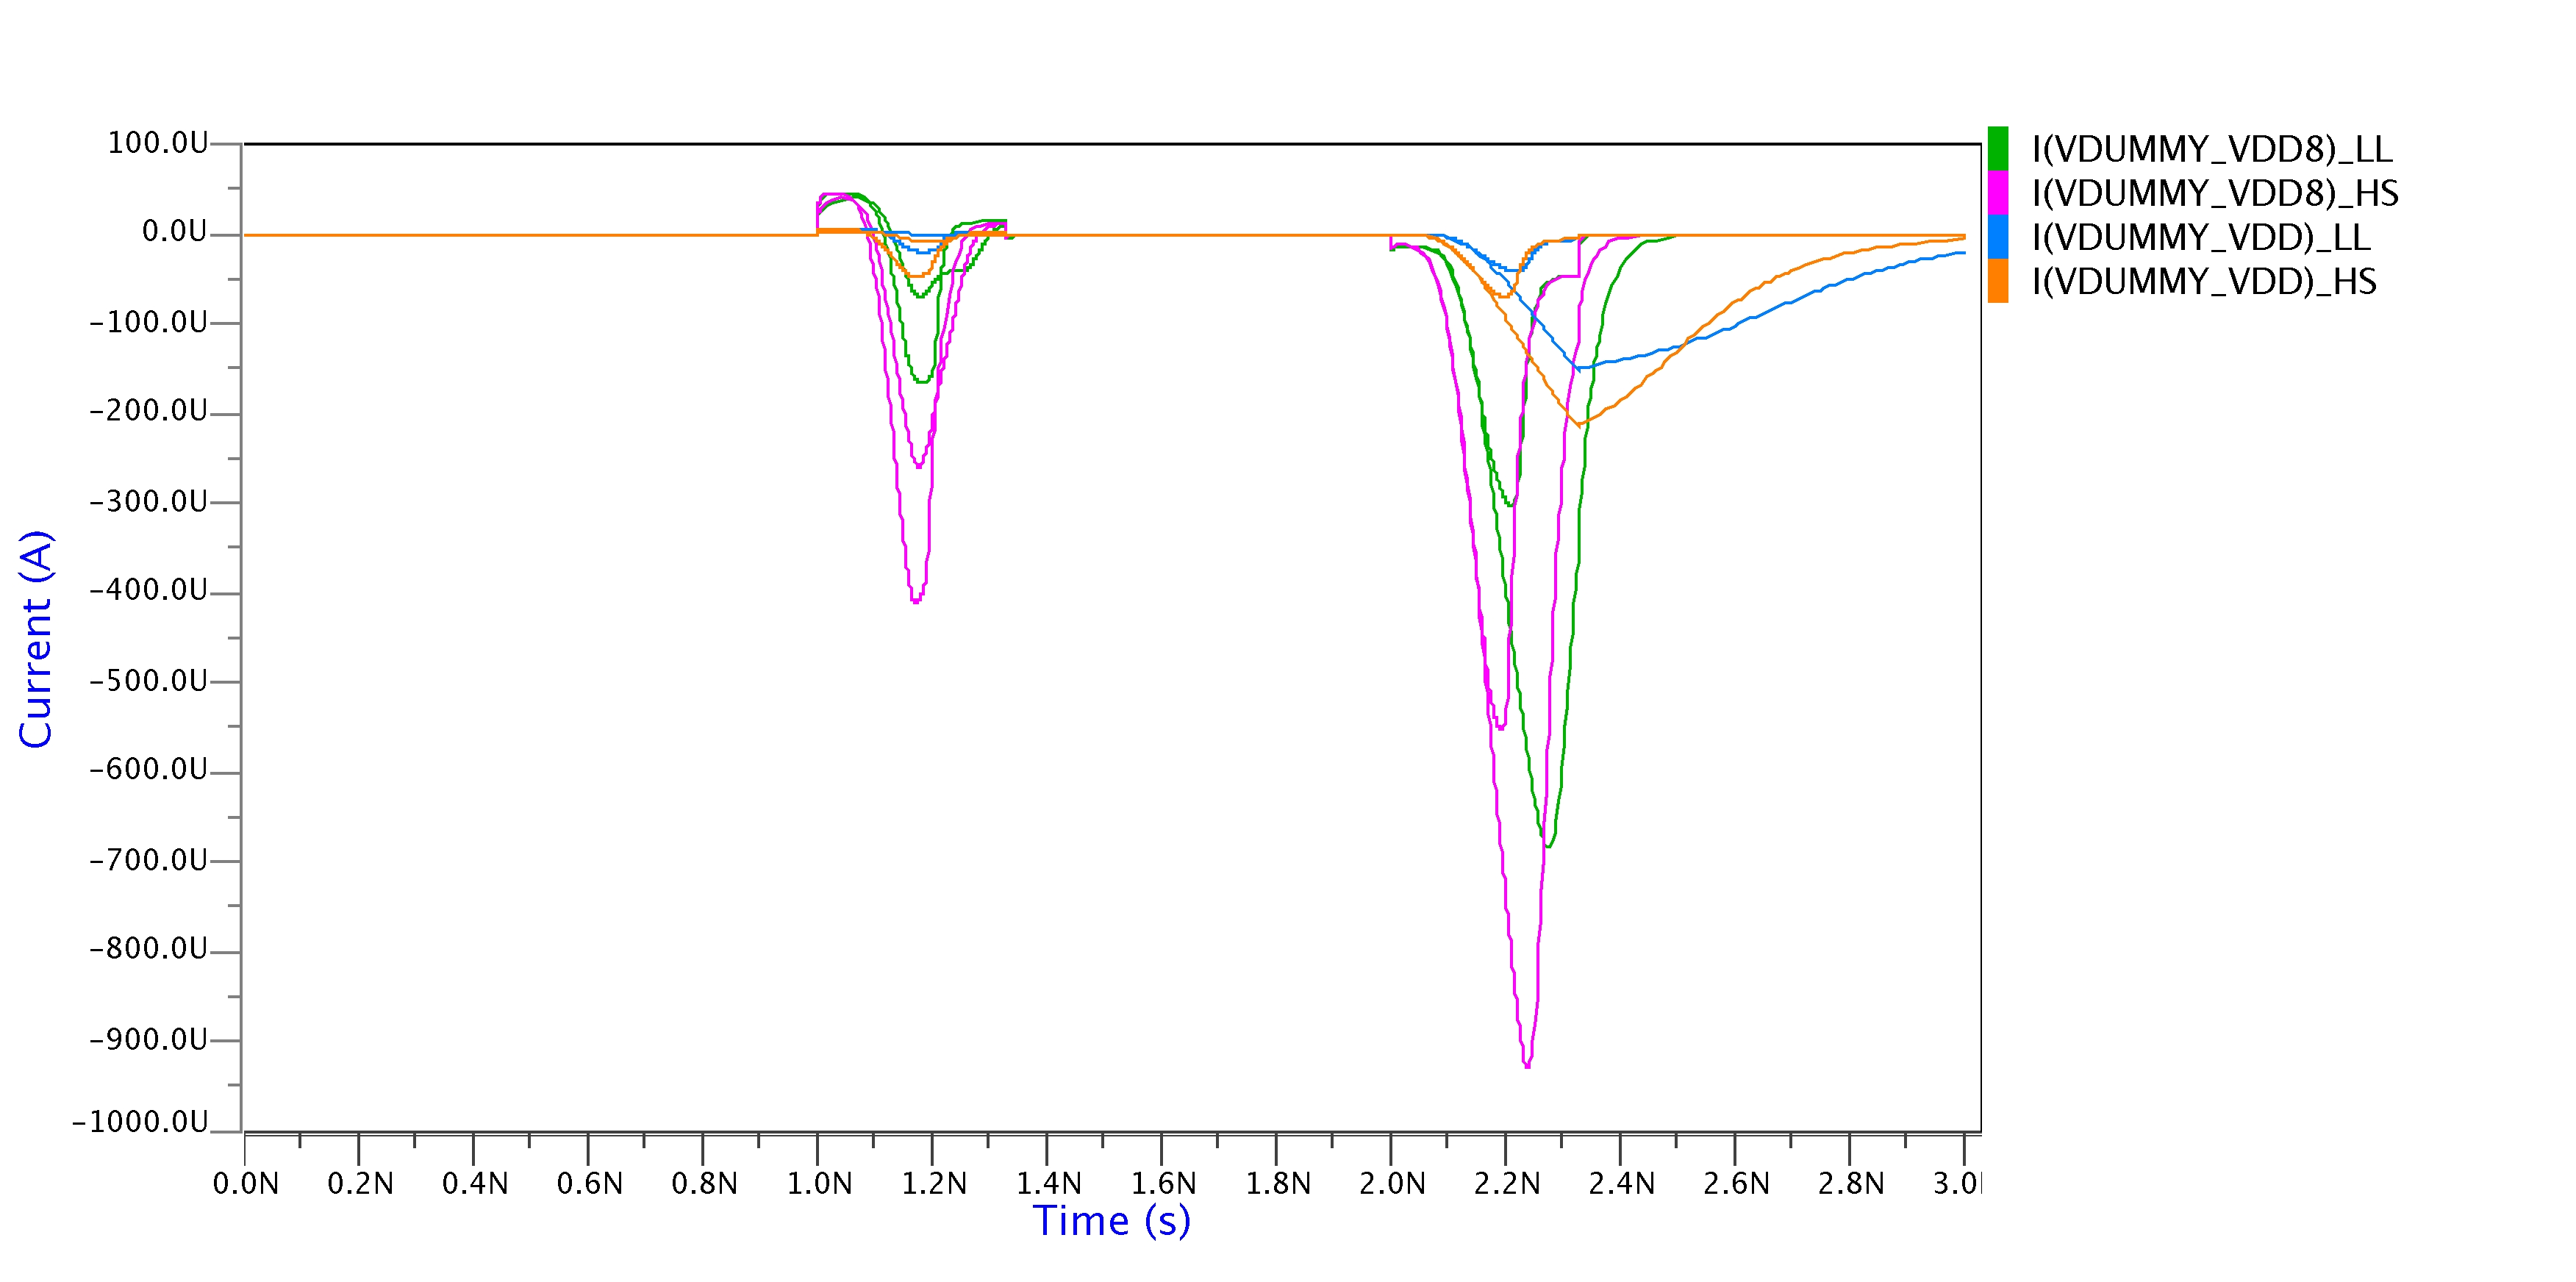
\includegraphics[scale=0.12]{immagini/onde_5_4_current3}
	\caption{\textit{Schema circuitale porta NAND}}
	\label{onde_5_4_current3}
\end{figure}
\noindent Infine, sempre tramite la simulazione ELDO, si è andata a stimare la potenza totale dissipata che è risultata essere pari a:
\begin{center}
	$Total Power Dissipation X8 = 2.9686 nW $ \\
	$Total Power Dissipation X1 = 445.09 pW $
\end{center}
Andando a confrontare questi valori con quelli ottenuti nel punto precedente, si può notare come la potenza si sia ridotta drasticamente. Precisamente si è ottenuta una riduzione del 93.99\% nel caso del gate X8 e del 93.44\% nel caso del gate X1.

\section{Temperature dependency}
In questa sezione si è andato a studiare l'andamento della potenza e della tensione di soglia, al variare della temperatura. Andando a modificare leggermente lo script, commentando il valore di capacità di 0.06 pF e inserendo un particolare comando \textit{.temp -40 0 40 80 120 150 180}, si ottiene una simulazione ELDO dove posso andare a vedere come varia la potenza in funzione della temperatura. I dati sono stati raccolti nella Tabella \ref{Tab5_23}.
\begin{table}[!h]\footnotesize
	\centering
	\begin{tabular}{|c|c|}
		\hline
		\textbf{Temperatura}&\textbf{Potenza}\\
		\hline
		-40°C&0.011197 nW\\
		0°C&0.12121 nW\\
		40°C&0.76913 nW\\
		80°C&3.2020 nW\\
		120°C&9.8880 nW\\
		150°C&19.907 nW\\
		180°C&36.351 nW\\
		\hline
	\end{tabular}
	\caption{\textit{Tensioni di soglia}}
	\label{Tab5_23}
\end{table}
\\
Infine, tramite il programma \textbf{gnuplot} ed uno script appositamente realizzato, si ottiene un preciso plot che mostra l'andamento della potenza in funzione della temperatura. Il grafico è riportato in Figura \ref{TEMP}.
\begin{figure}[!htb]
	\centering
	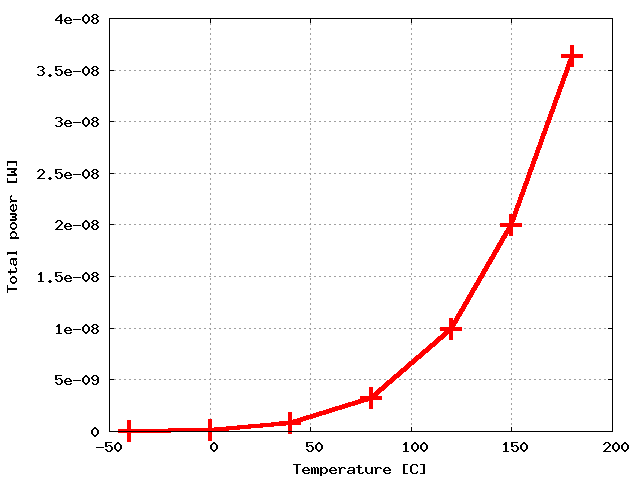
\includegraphics[scale=0.55]{immagini/TEMP}
	\caption{\textit{Schema circuitale porta NAND}}
	\label{TEMP}
\end{figure}
\\
Allo stesso modo si è andato a simulare il comportamento della Tensione di Soglia al variare della Temperatura. I dati sono raccolti nella Tabella \ref{Tab5_24} e il grafico è presente in Figura \ref{TEMPVT}
\begin{table}[!h]\footnotesize
	\centering
	\begin{tabular}{|c|cccc|}
		\hline
		&\textbf{Tensione di Soglia} \textbf{$V_{TH}$}&&&\\
		\hline
		\textbf{Temperatura}&\textbf{XMN0.M1}&\textbf{XMN1.M1}&\textbf{XMP0.M1}&\textbf{XMP1.M1}\\
		\hline
		-40°C&0.45753&0.42482&-0.41556&-0.41556\\
		0°C&0.43114&0.39843&-0.38664&-0.38664\\
		40°C&0.40476&0.37204&-0.35772&-0.35772\\
		80°C&0.37837&0.34566&-0.32880&-0.32880\\
		120°C&0.35199&0.31927&-0.29988&-0.29988\\
		150°C&0.33220&0.29949&-0.27819&-0.27819\\
		180°C&0.31241&0.27970&-0.25650&-0.25650\\
		\hline
	\end{tabular}
	\caption{\textit{Tensioni di soglia}}
	\label{Tab5_24}
\end{table}
\begin{figure}[!htb]
	\centering
	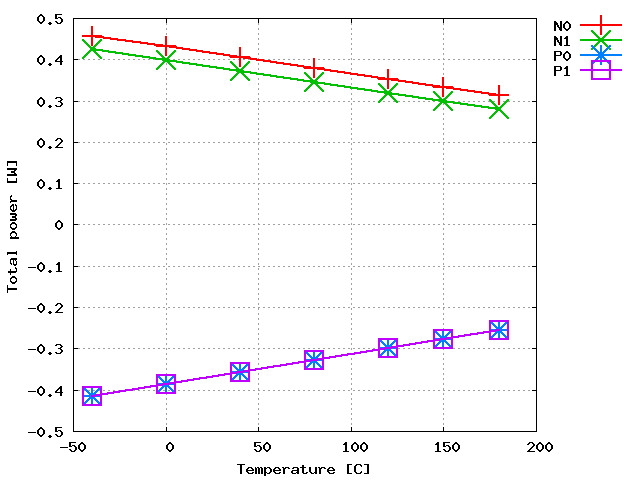
\includegraphics[scale=0.55]{immagini/TEMPVT}
	\caption{\textit{Schema circuitale porta NAND}}
	\label{TEMPVT}
\end{figure}

SERVONO DEI COMMENTI??????? PORCA TROIA I COMMENTI

\section{Analysis of a memory power components}
Lo scopo di quest’ultimo punto dell’esercitazione è  analizzare i datasheet delle varie versioni di memoria fornite e scegliere la migliore struttura di memoria che ottimizzi i consumi di potenza. Infatti dal punto di vista dei consumi è molto più conveniente dividere la struttura della memoria in banchi in modo da ridurre il numero di celle coinvolte nell’operazione di accesso alla memoria. 
La memoria da progettare deve avere la stessa capienza di una SRAM\_8192\_16\_16, con varie possibilità di scelta del parallelismo e delle dimensioni.
Dopo aver scelto un parallelismo a 16 bit, si è andato ad analizzare il consumo delle varie memorie tramite i vari contributi di corrente con la formula fornita nella user guide delle SRAM a 90 nm:
\begin{center}
$Itot= Iavg+Ides*Ndes$
\end{center}
\begin{center}
	$Iavg=Isw+Isby+½*(cout*Val*f*Nb*Np)$
\end{center}
dove:
\begin{itemize}
\item $I_{DES}$ è la corrente che scorre nella cella non selezionata
\item $N_{DES}$ è il numero di celle non selezionate ( $16-1=15$ )
\item $I_{sw}$ è il valore medio della corrente durante le fasi di scrittura e lettura
\item $I_{sby}$ è la corrente che scorre nella cella quando i segnali di ingresso e di uscita sono stabili
\item $C_{out}$ è il valore della capacità di carico in uscita, scelta uguale per tutte le memorie visto che il valore non è noto a priori ($1pF$)
\item $V_{al}$ è la tensione di alimentazione per il caso tipico, $1V$
\item $f$ è la frequenza operativa ($1MHz$)
\item $N_{bits}$ è il numero di bit in uscita ($16$)
\item $N_{ports}$ è il numero di porte della memoria scelta ($2$, memoria dual-port)
\end{itemize}
Sono quindi state analizzate tutte le memorie con parallelismo a 16 bit così da confrontarne i consumi in termini di corrente totale, trascurando i consumi dei multiplexer di uscita.
\begin{table}[!h]\footnotesize
	\centering
	\begin{tabular}{|c|c|c|c|c|c|c|}
		\hline
		\textbf{Memory} & \textbf{$I_{sw}$ $\mu A$}& \textbf{$I_{sby}$ $\mu A$} & \textbf{$I_{des}$ $\mu A$} & \textbf{$N_{bits}$ $\mu A$} & \textbf{$N_{blocks}$ $\mu A$} &
		\textbf{$I_{tot}$ $\mu A$}
		\\
		\hline
		SRAM 256\_16\_4 & 7.27 & 82 &2.7 & 4 & 32 & 189\\
		SRAM 512\_16\_4 & 7.70 & 118 & 2.8 &  4 & 16 & 184\\
		SRAM 512\_16\_16 & 10.8 & 156 & 5.21 & 16 & 16 & 261\\
		SRAM 1024\_16\_4 & 8.34 & 190 & 2.79 & 4 & 8 & 234\\
		SRAM 1024\_16\_16 & 11.2 & 181 & 5.51 & 16 & 8 & 247\\
		SRAM 2048\_16\_16 & 11.8 & 232 & 5.71 & 16 & 4 & 277\\
		SRAM 4096\_16\_16 & 12.4 & 333 & 5.68 & 16  & 2 & 367\\
		\hline
	\end{tabular}
	\caption{\textit{Caratteristiche delle SRAM analizzate.}}
	\label{Tab5_25}
\end{table}
\\
\\
Dalla tabella si evince che la formula più conveniente con questo parallelismo è una memoria formata da 16 blocchi di  SRAM 512\_16\_4, formata da 512  words  di 16 bit con profondità dei multiplexer uguale a 4, che consuma una corrente totale di circa 184 uA.
